\label{Beispiele}
\chapter{Beispielsitzung}

	Auf den nächsten Seiten sind einige Bildschirmabzüge des Coaching Bots zu sehen. Zunächst wird durch eine Sitzung aus Sicht des Nutzers geführt, bevor die Ansicht des Coaches gezeigt wird.\\ 
	\\
	\begin{enumerate}
		\item Abb. 7.1 (a): Der Nutzer startet den Bot via einem Klick auf einen Link\footnote{\url{https://t.me/thecoachingbot?start=start}}, den er auf einer Website findet oder der ihm zugesandt wird.
		\item Abb. 7.1 (b): Im Telegram-Bot angekommen, sieht man unten einen Butten \textbf{Starten}. Auf diesen tipt der Nutzer und die Konversation mit dem Bot wird gestartet.
		\item Abb. 7.2 (a): Der Nutzer wird begrüßt, es wird kurz erklärt, wie man den Bot beendet und daraufhin wird die erste Frage nach einigen Informationen zum Nutzer gestellt.
		\item Abb. 7.2 (b): Nach der Beantwortung der Frage, antwortet der Bot auf diese und stellt die Nächste. Da für die Auswahl des Geschlechts nur vordefinierte Antworten vorgesehen sind, werden diese in einer entsprechend konfigurierten Tastatur dargestellt. Tipt der Nutzer auf eine der drei Optionen, so gelangt er zu Frage nach dem Geburtsdatum. Die Stufe kann übersprungen werden.
		\item Abb. 7.3 (a): Sein Geburtsdatum kann der Nutzer nun angeben, allerdings nur im prädefinierten Format. Tut er dies korrekt oder gibt /skip ein, gelangt er zur nächsten Stufe. Ansonsten wird er darauf hingewiesen, dass die Eingabe inkorrekt war und kann es noch einmal versuchen. 
		\item Abb. 7.3 (b): Der Nutzer wird nun nach seiner E-Mail-Adresse gefragt. Auch hier muss die Adresse einem handelsüblichen E-Mail-Format entsprechen. Da dieses Format aber allgemeinhin bekannt ist, wird es hier nicht explizit angezeigt. Die Stufe kann nicht übersprungen werden. Man kann den Vorgang abbrechen oder eine korrekte E-Mail-Adresse eingeben.
		\item Abb. 7.4 (a): Damit ein Telefongespräch zwischen Coach und Coachee zustande kommt, wird nun nach der Telefonnummer gefragt. Diese sollte korrekt, muss aber nicht zwingend angegeben werden. Auch hier liegt eine Validierung hinter der Eingabe. Ein Kontakt zum Nutzer kann auch später via E-Mail oder Anpassung der Termineinladung erfolgen. 
		\item Abb. 7.4 (b): Der Nutzer hat hier die Möglichkeit, seinen Standort via der integrierten Standortfreigabe zu teilen. Dies ist rein optional. Ein Überspringen via /skip wird aus Rücksicht auf die Privatsphäre angeboten. 
		\item Abb. 7.5 (a): Dem Nutzer wird ein stilisiertes Bild ausgegeben, das den Bot repräsentieren soll. So wird der Nutzer dazu angeleitet, auch ein Bild von sich zu teilen. Die Stufe kann übersprungen werden.
		\item Abb. 7.5 (b): Hat der Nutzer sein Bild geteilt, registriert der Bot, dass alle Stufen erfolgreich abgeschlossen oder übersprungen wurden und damit die Kriterien für den Abschluss des Anmeldeprozesses erfüllt sind. Er bietet dem Nutzer nun in einer prädefinierten Tastatur an, den Prozess abzuschließen und einen Termin zu vereinbaren oder seine Daten wieder zu löschen.
		\item Abb. 7.6 (a): Hat der Nutzer sich entschieden, einen Termin zu vereinbaren, so wird ihm zunächst eine Übersicht über angegebene Kontaktdaten angezeigt und suggeriert, dass der Bot nun nach verfügbaren Terminen sucht. Das passiert auch im Hintergrund.
		\item Abb. 7.6 (b): Sobald der Bot drei freie Termine gefunden hat, schlägt er dem Nutzer diese in einer dynamischen Tastatur vor. Der Nutzer kann nun wählen, welchen Termin er vereinbaren möchte oder die Sitzung verlassen.
		\item Abb. 7.7 (a): Entscheidet der Nutzer sich dazu, einen Termin zu vereinbaren, so bestätigt der Bot diesen und gibt Bescheid, dass der Coachee zur entsprechenden Zeit vom Coach angerufen wird. 
		\item Abb. 7.7 (b): Fast gleichzeitig trifft beim Nutzer eine Termineinladung via E-Mail oder Calender-Client ein und kann - je nachdem, wie der Nutzer sein System konfiguriert hat - direkt akzeptiert oder abgelehnt werden. Informationen über die Art des Termins und die Telefonnummer des Nutzers sind bereits im Termin enthalten. Damit ist die Haupt-User-Journey beendet.
		\item Abb. 7.8 (a): Sollte der Nutzer nach Vereinbarung des Termins wieder zum Bot zurückkehren, dann werden ihm Termin sowie die Möglichkeit angezeigt, dass er diesen jederzeit in seinem Kalender wieder ablehnen kann. Außerdem kann er natürlich jederzeit seine Daten löschen oder den Status abfragen.
		\item Abb. 7.8 (b): Verlässt der Nutzer den Bot und kehrt erst nach einiger Zeit wieder zu ihm zurück oder möchte aus einem anderen Grund wissen, wie viele Fragen er schon beantwortet hat, so kann er dies via dem Befehl /status tun. Es wird ausgegeben, wie viele von wie vielen Stufen bereits durchlaufen worden sind. Möchte der Nutzer aufgezeigt bekommen, welche Interaktionsmöglichkeiten es mit dem Bot gibt, so kannn er jederzeit den Befehl /hilfe eingeben. Die Hilfe mit allen Befehlen und einer kurzen Erklärung wird ausgegeben.
		\item Abb. 7.9 (a): Entscheidet der Nutzer sich zu einem beliebigen Zeitpunkt, seine Daten zu löschen, so kann er dies über den Befehl /delete veranlassen. Ist der Prozess erfolgreich, wird ihm das bestätigt. (Ansonsten wird ein Fehler ausgegeben.) Danach ist der Nutzer dem Bot wieder vollkommen unbekannt. Ein Neustart des Konversationsflusses ist also sofort und ohne Weiteres möglich.
		\item Abb. 7.10: Der Coach hat hier die Möglichkeit, all seine Termine in einer Monats-Kalender-Übersicht sowie alle Anmeldungen in einer Listenform einzusehen. 
		
	\end{enumerate}
	

	% PAGE 01
	\begin{figure}
		\centering
		\begin{minipage}{.48\linewidth}
		  \centering
		  \subcaptionbox{Einstieg via URL}
			{
\includegraphics[width=\linewidth,height=150pt,keepaspectratio]{images/Screenshots/link.png}}
	  
		  \subcaptionbox{Start des Coaching Bots}
			{
\includegraphics[width=\linewidth,height=300pt,keepaspectratio]{images/Screenshots/start.PNG}}
	  
		  \caption{Einstieg und Start}
		\end{minipage}\quad
		\begin{minipage}{.48\linewidth}
		  \centering
		  \subcaptionbox{Übergang zur Angabe der Biographie}
			{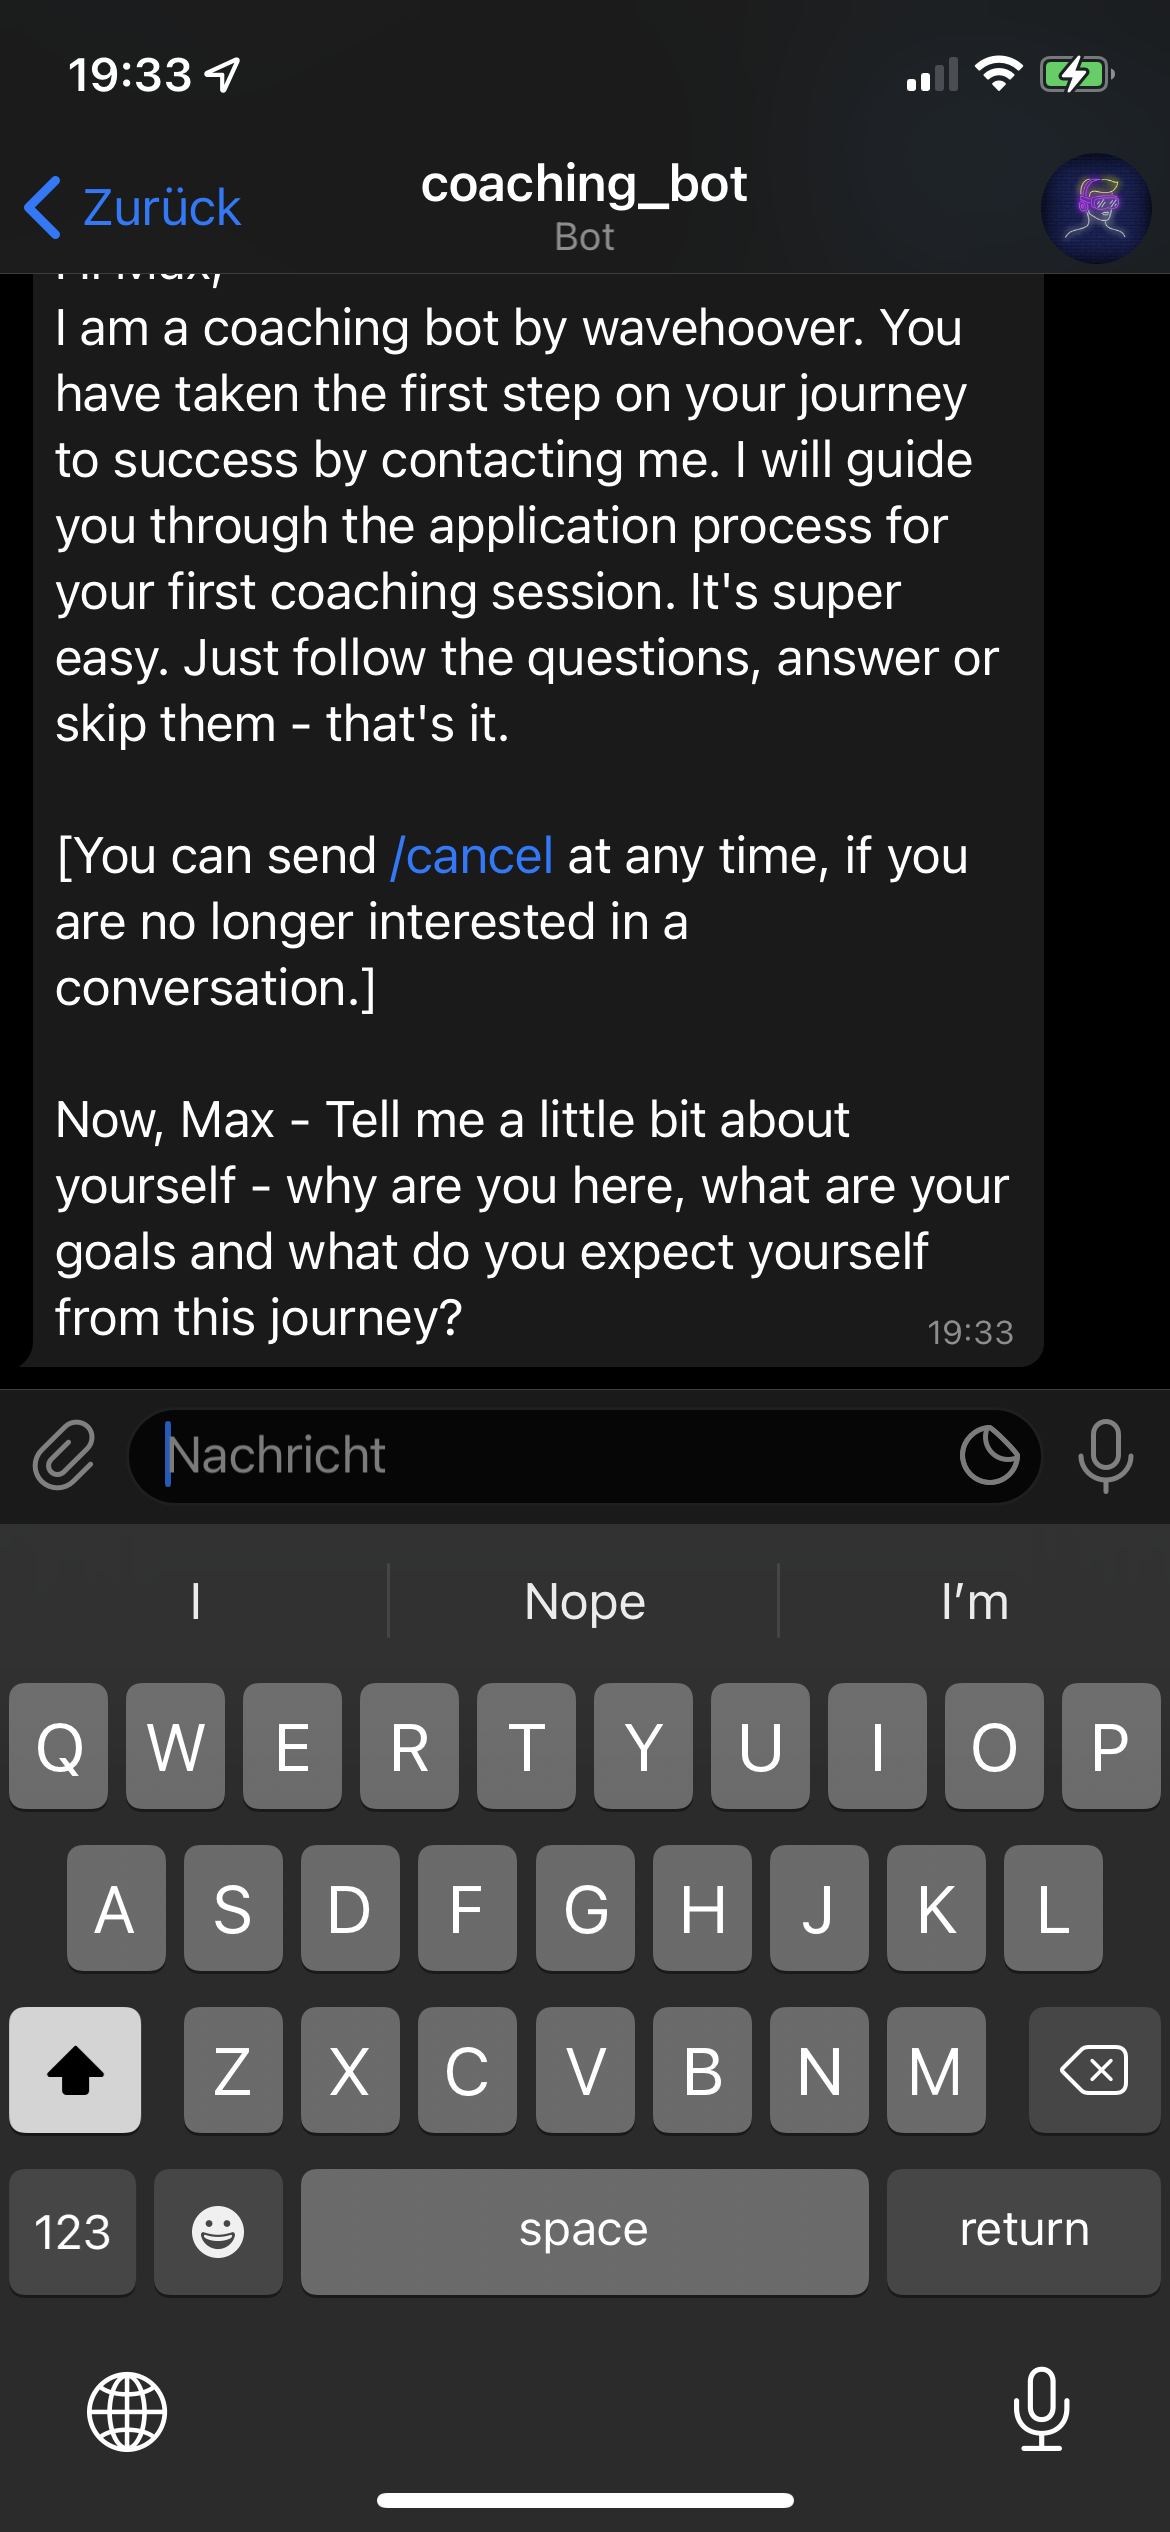
\includegraphics[width=\linewidth,height=300pt,keepaspectratio]{images/Screenshots/bio.PNG}}
	  
		  \subcaptionbox{Übergang zur Auswahl des Geschlechts}
			{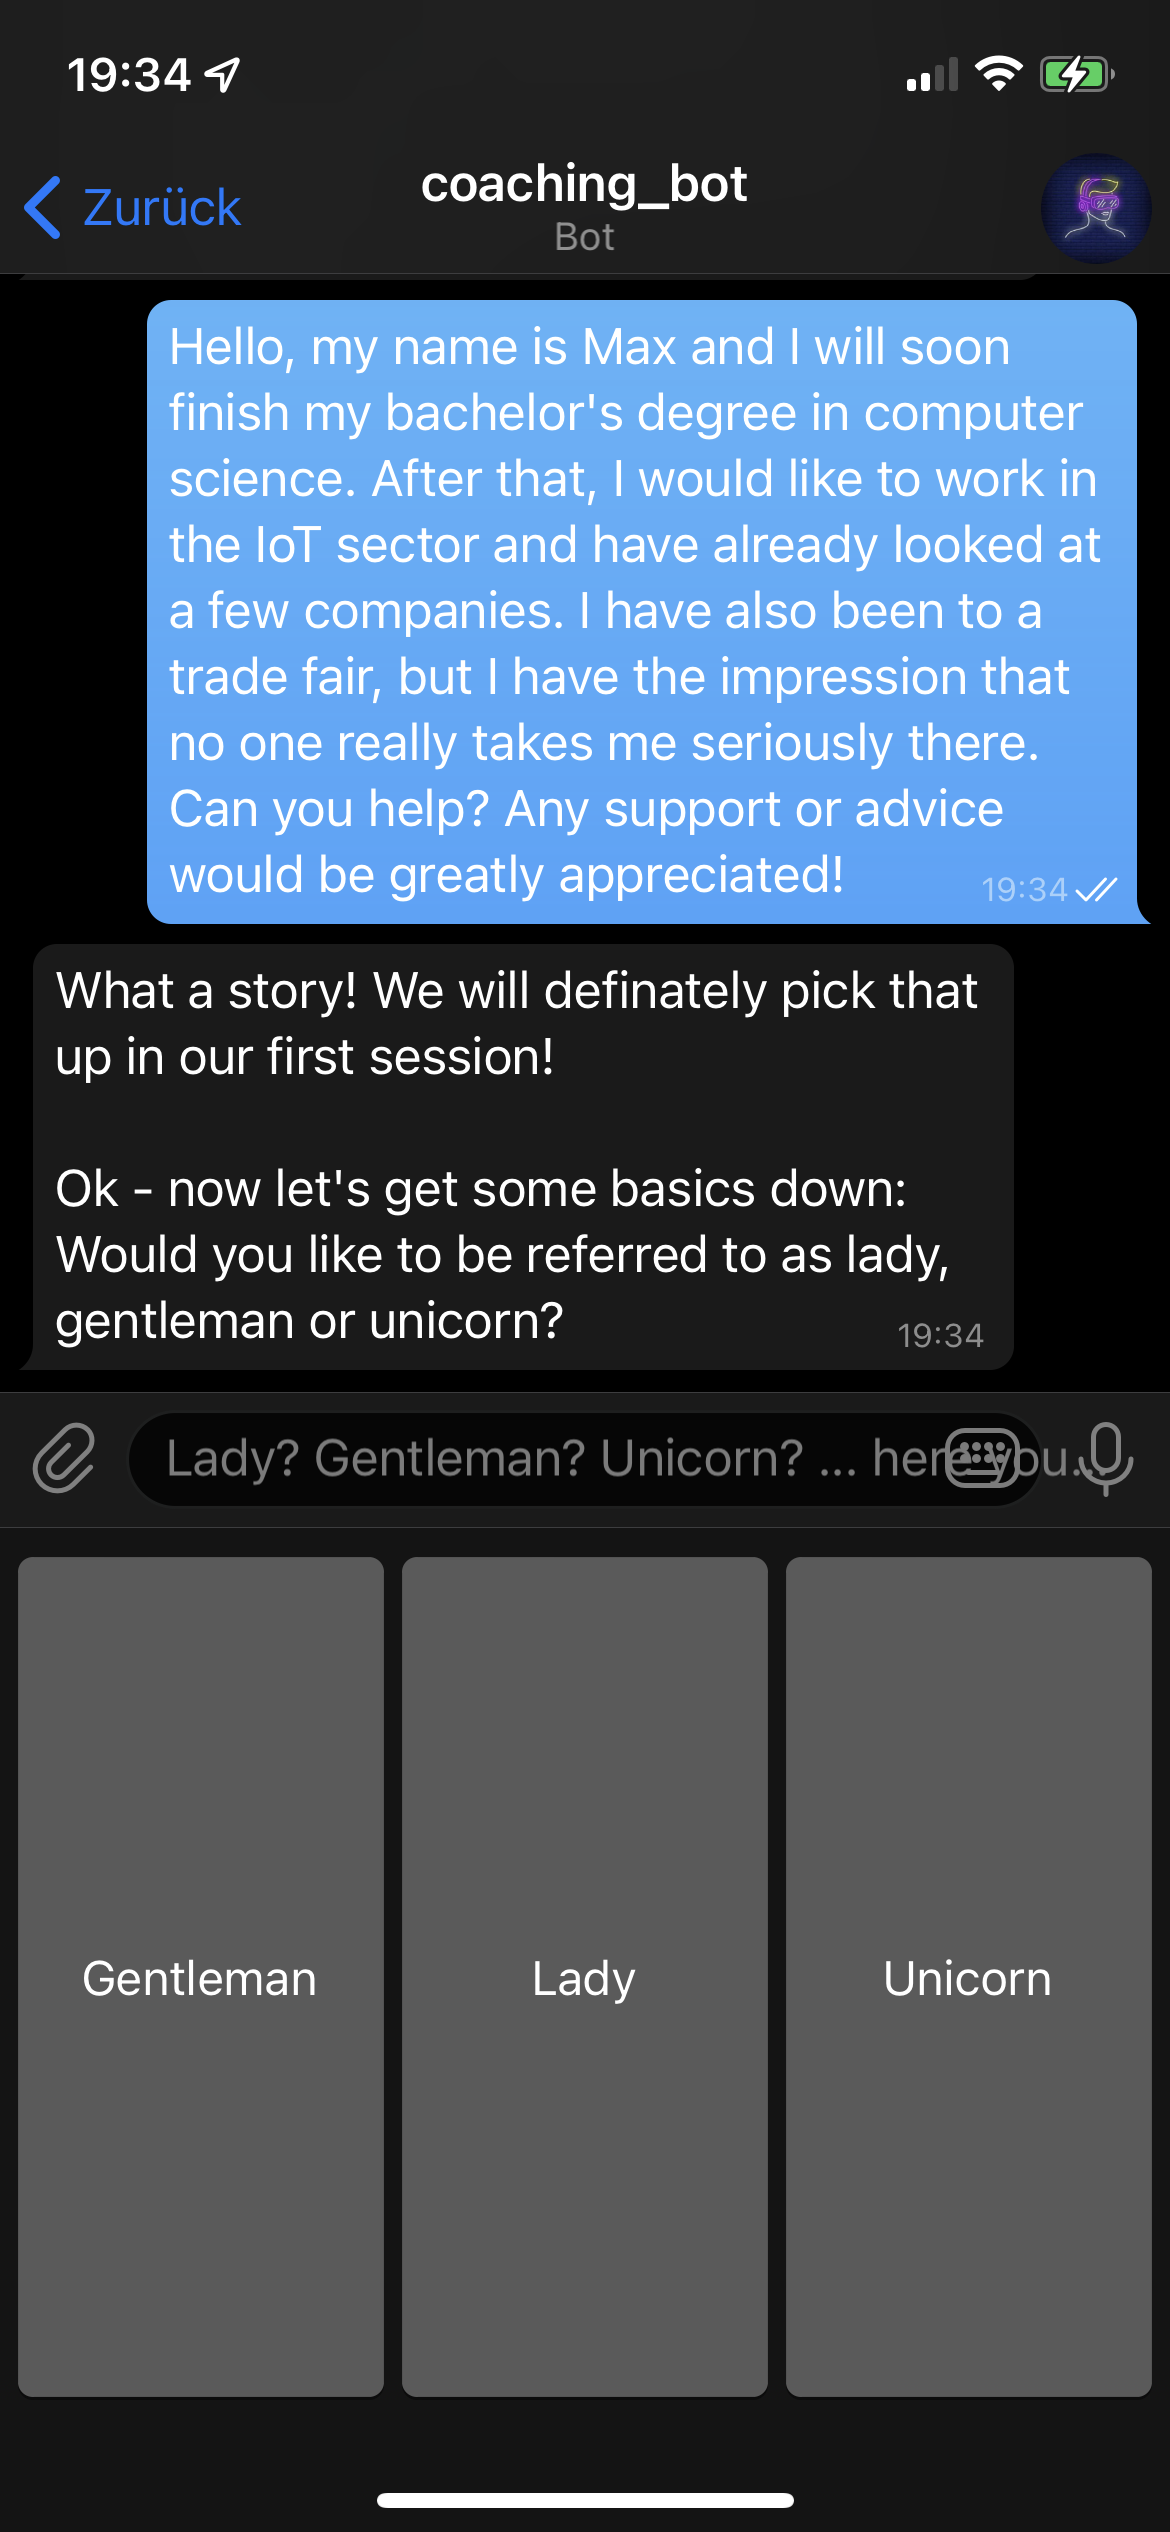
\includegraphics[width=\linewidth,height=300pt,keepaspectratio]{images/Screenshots/gender.PNG}}
	  
		  \caption{Erste Zustands-Übergänge}
		\end{minipage}
	\end{figure}


	% PAGE 02
	\begin{figure}
		\centering
		\begin{minipage}{.48\linewidth}
			\centering
			\subcaptionbox{Übergang zur Angabe des Geburtsdatums}
			{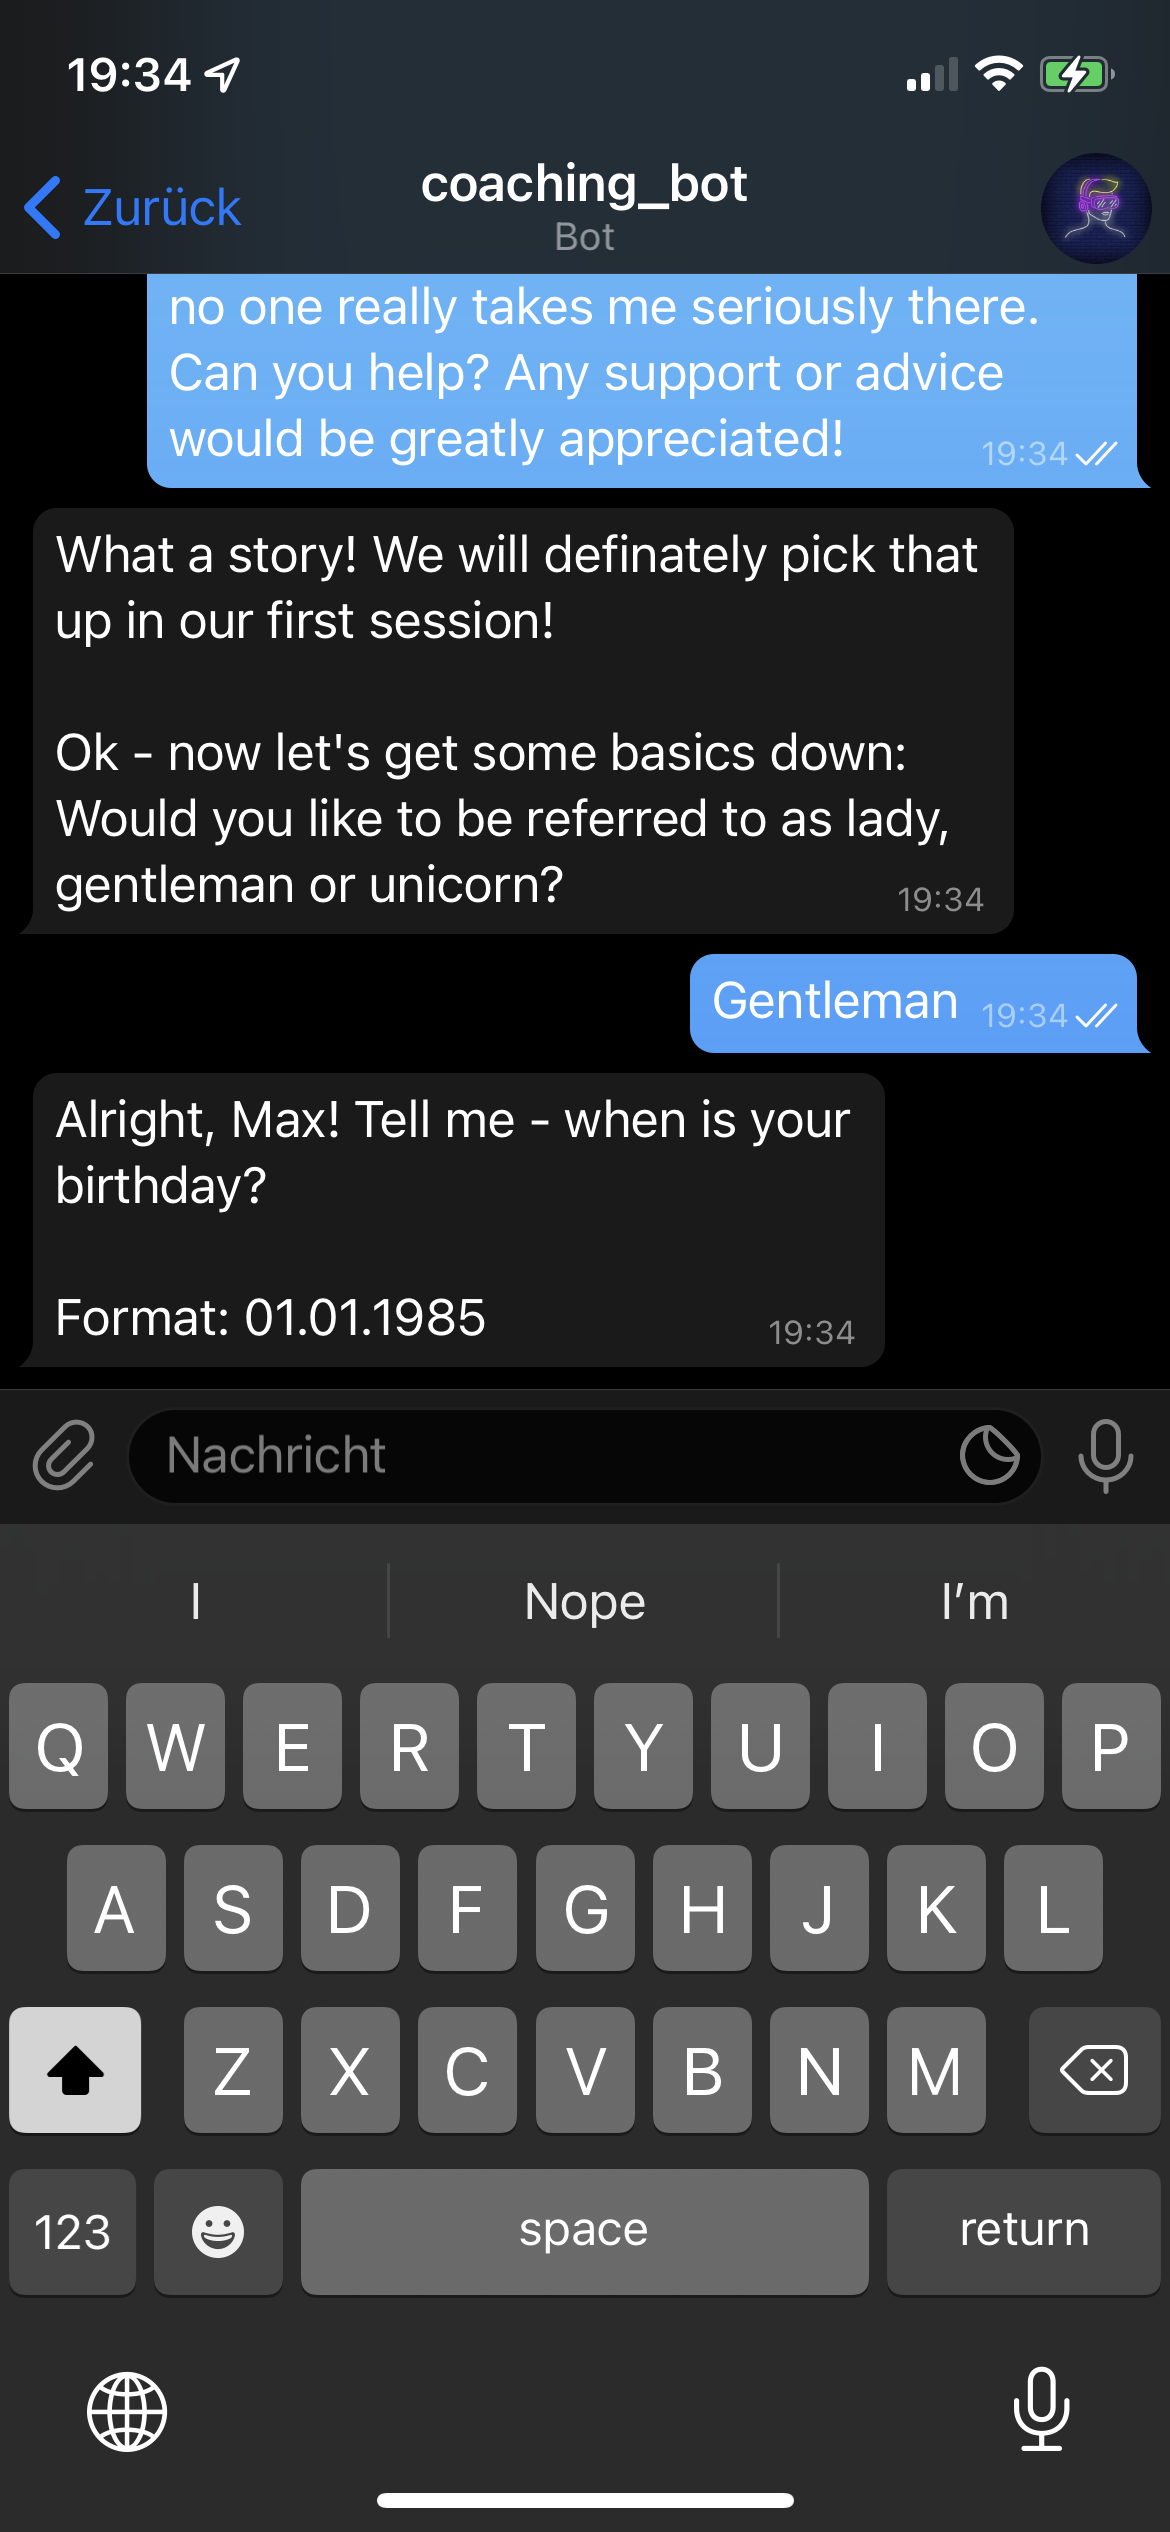
\includegraphics[width=\linewidth,height=300pt,keepaspectratio]{images/Screenshots/birthdate.PNG}}
		
			\subcaptionbox{Übergang zur Angabe der E-Mail-Adresse}
			{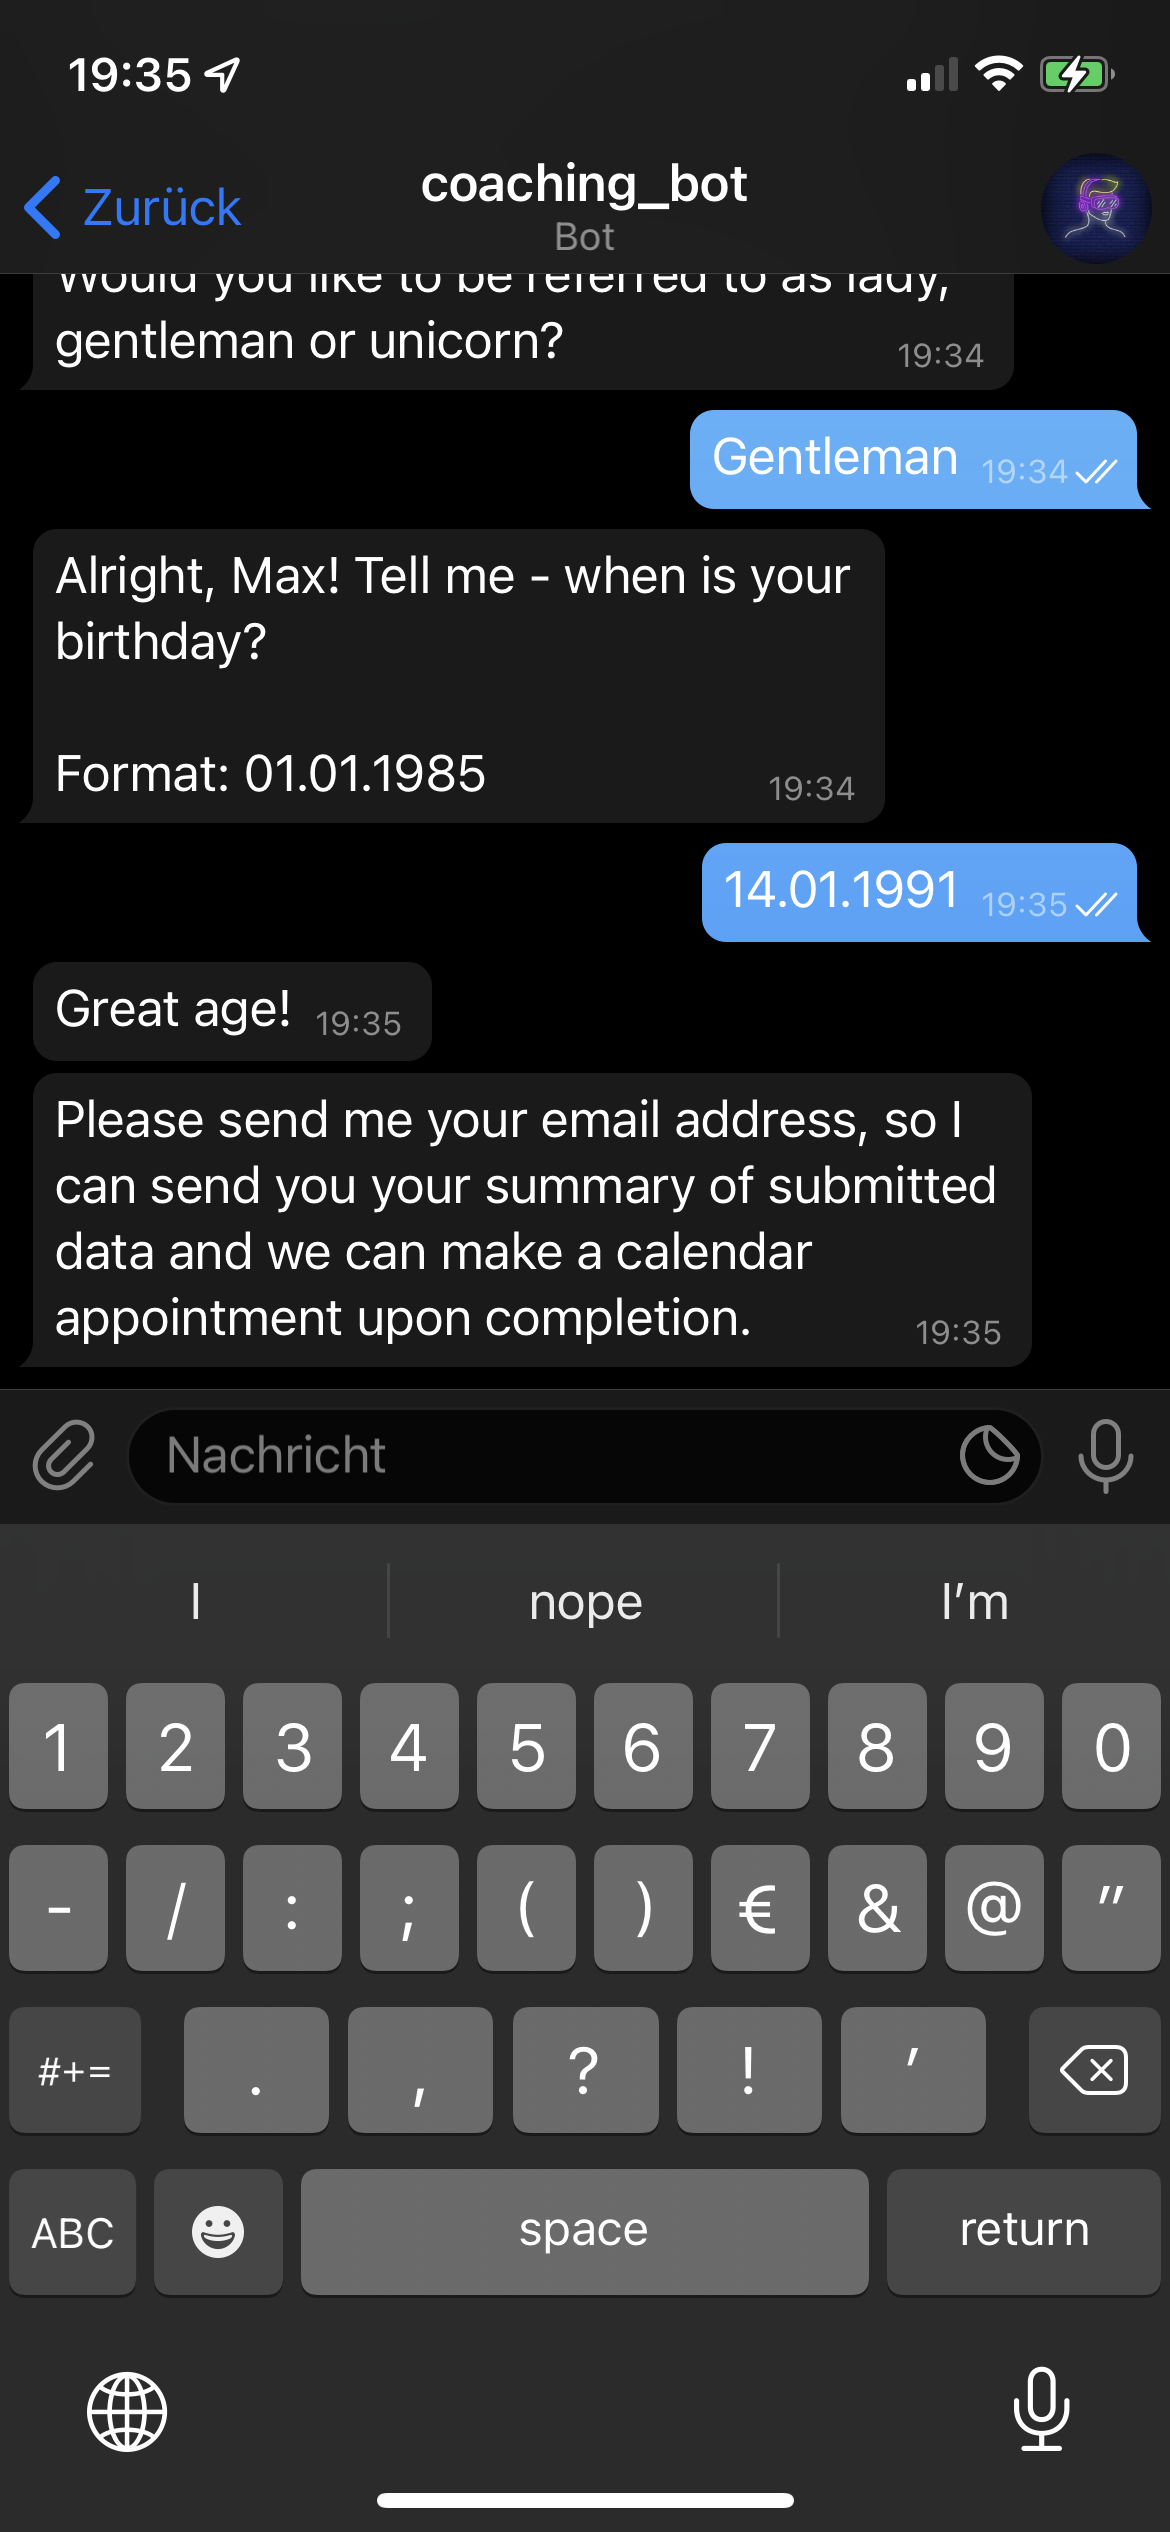
\includegraphics[width=\linewidth,height=300pt,keepaspectratio]{images/Screenshots/email.PNG}}
		
			\caption{Abfrage Geburtsdatum und E-Mail-Adresse}
		\end{minipage}\quad
		\begin{minipage}{.48\linewidth}
			\centering
			\subcaptionbox{Übergang zur Angabe der Telefonnummer}
			{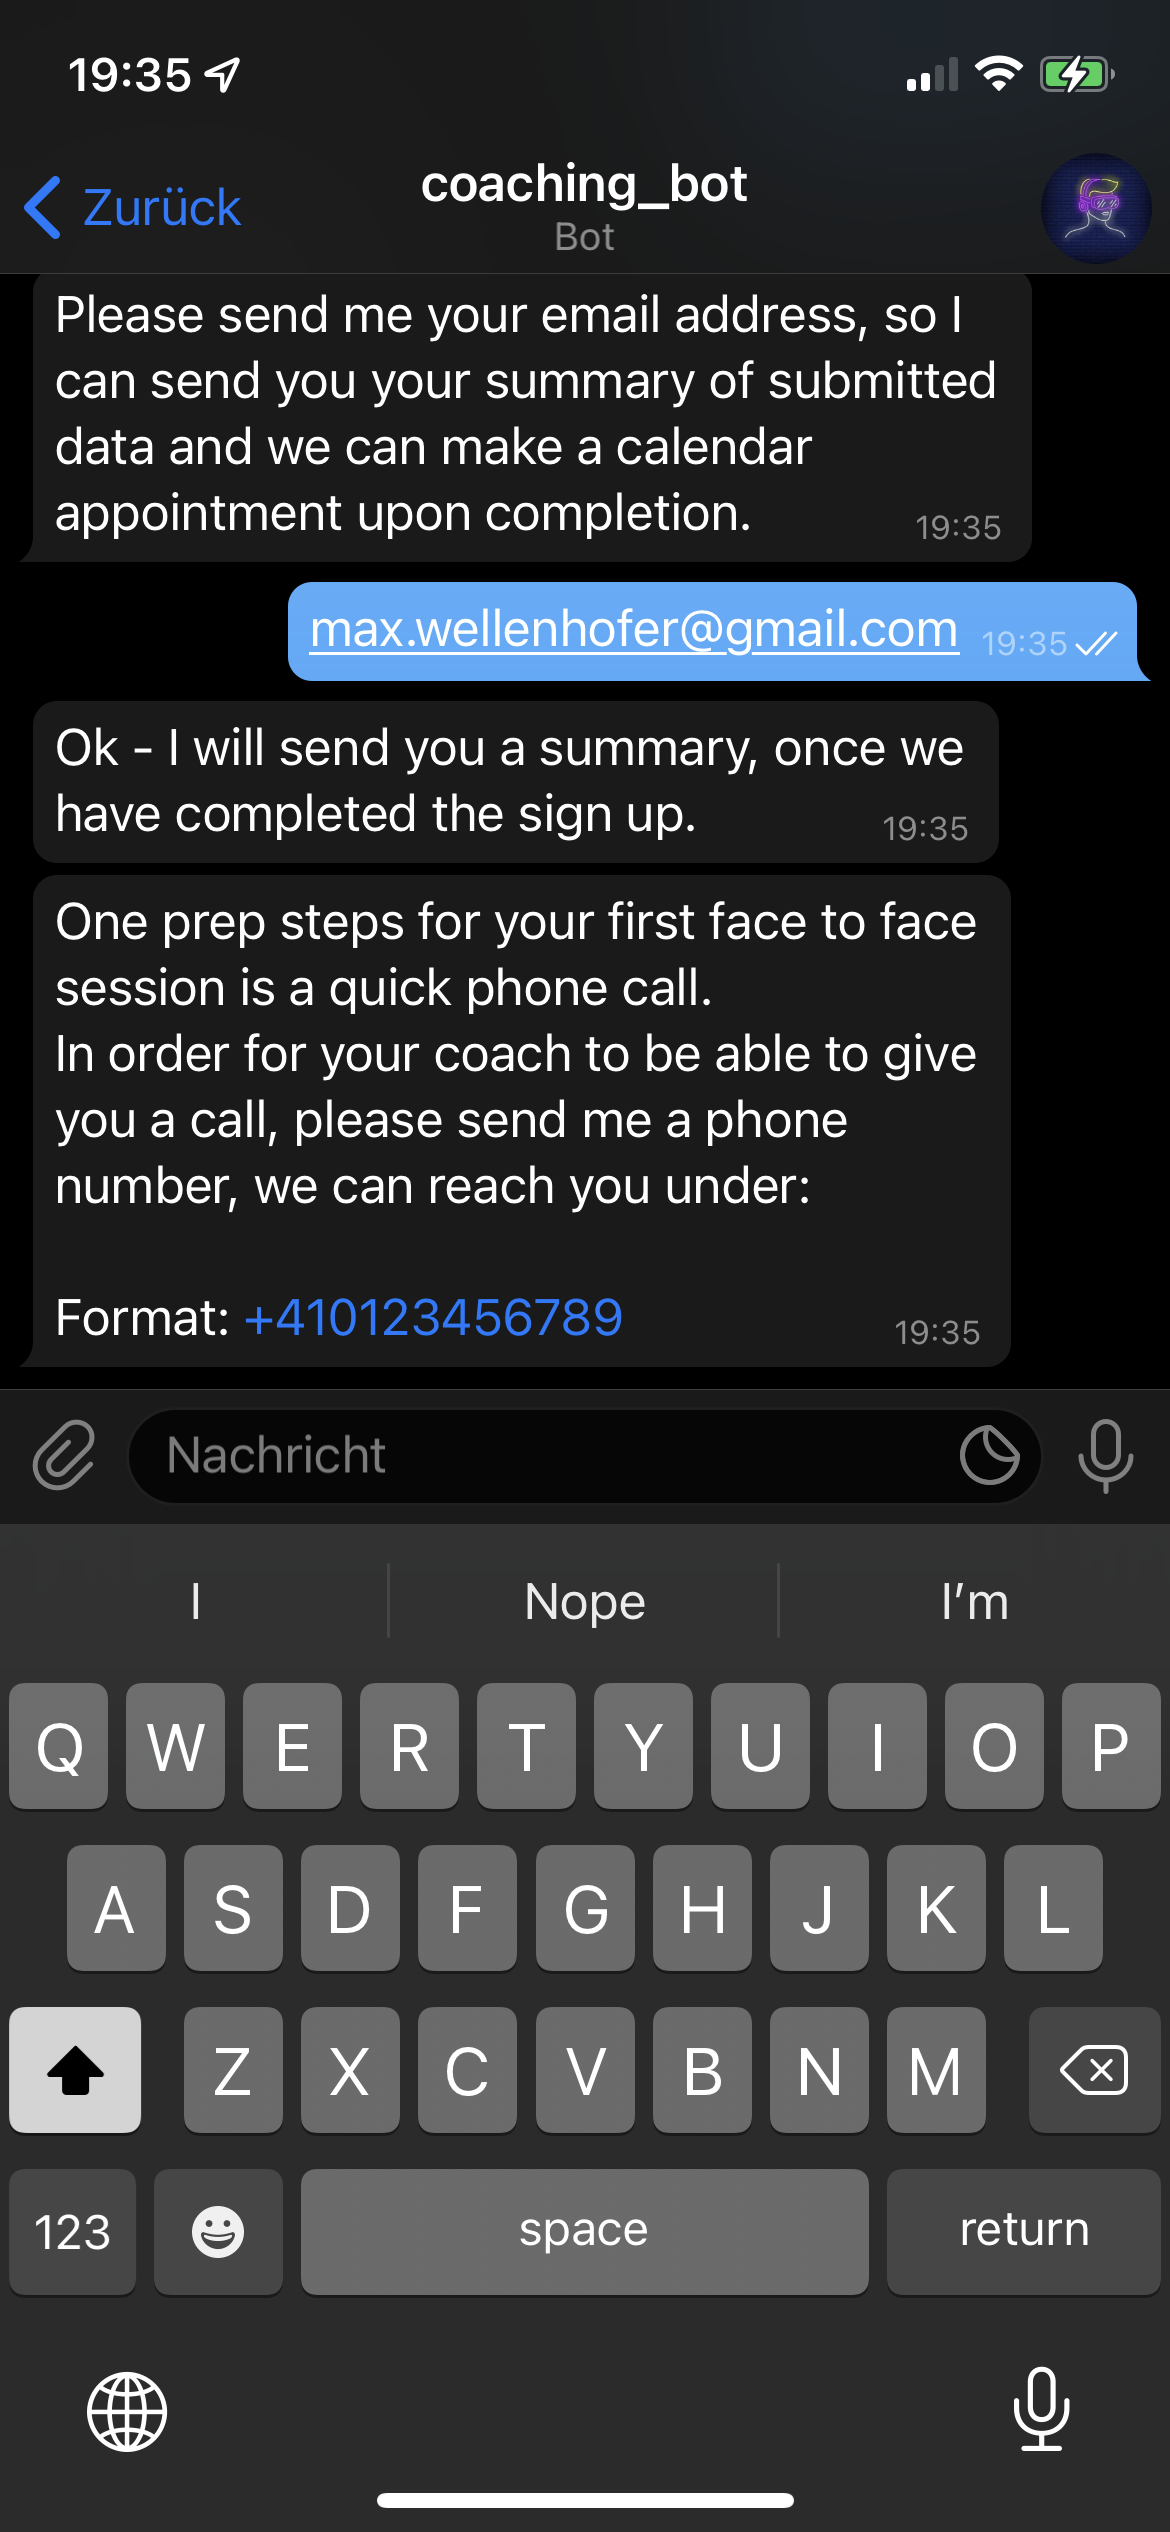
\includegraphics[width=\linewidth,height=300pt,keepaspectratio]{images/Screenshots/telephone.PNG}}
		
			\subcaptionbox{Übergang zur Angabe des Standorts}
			{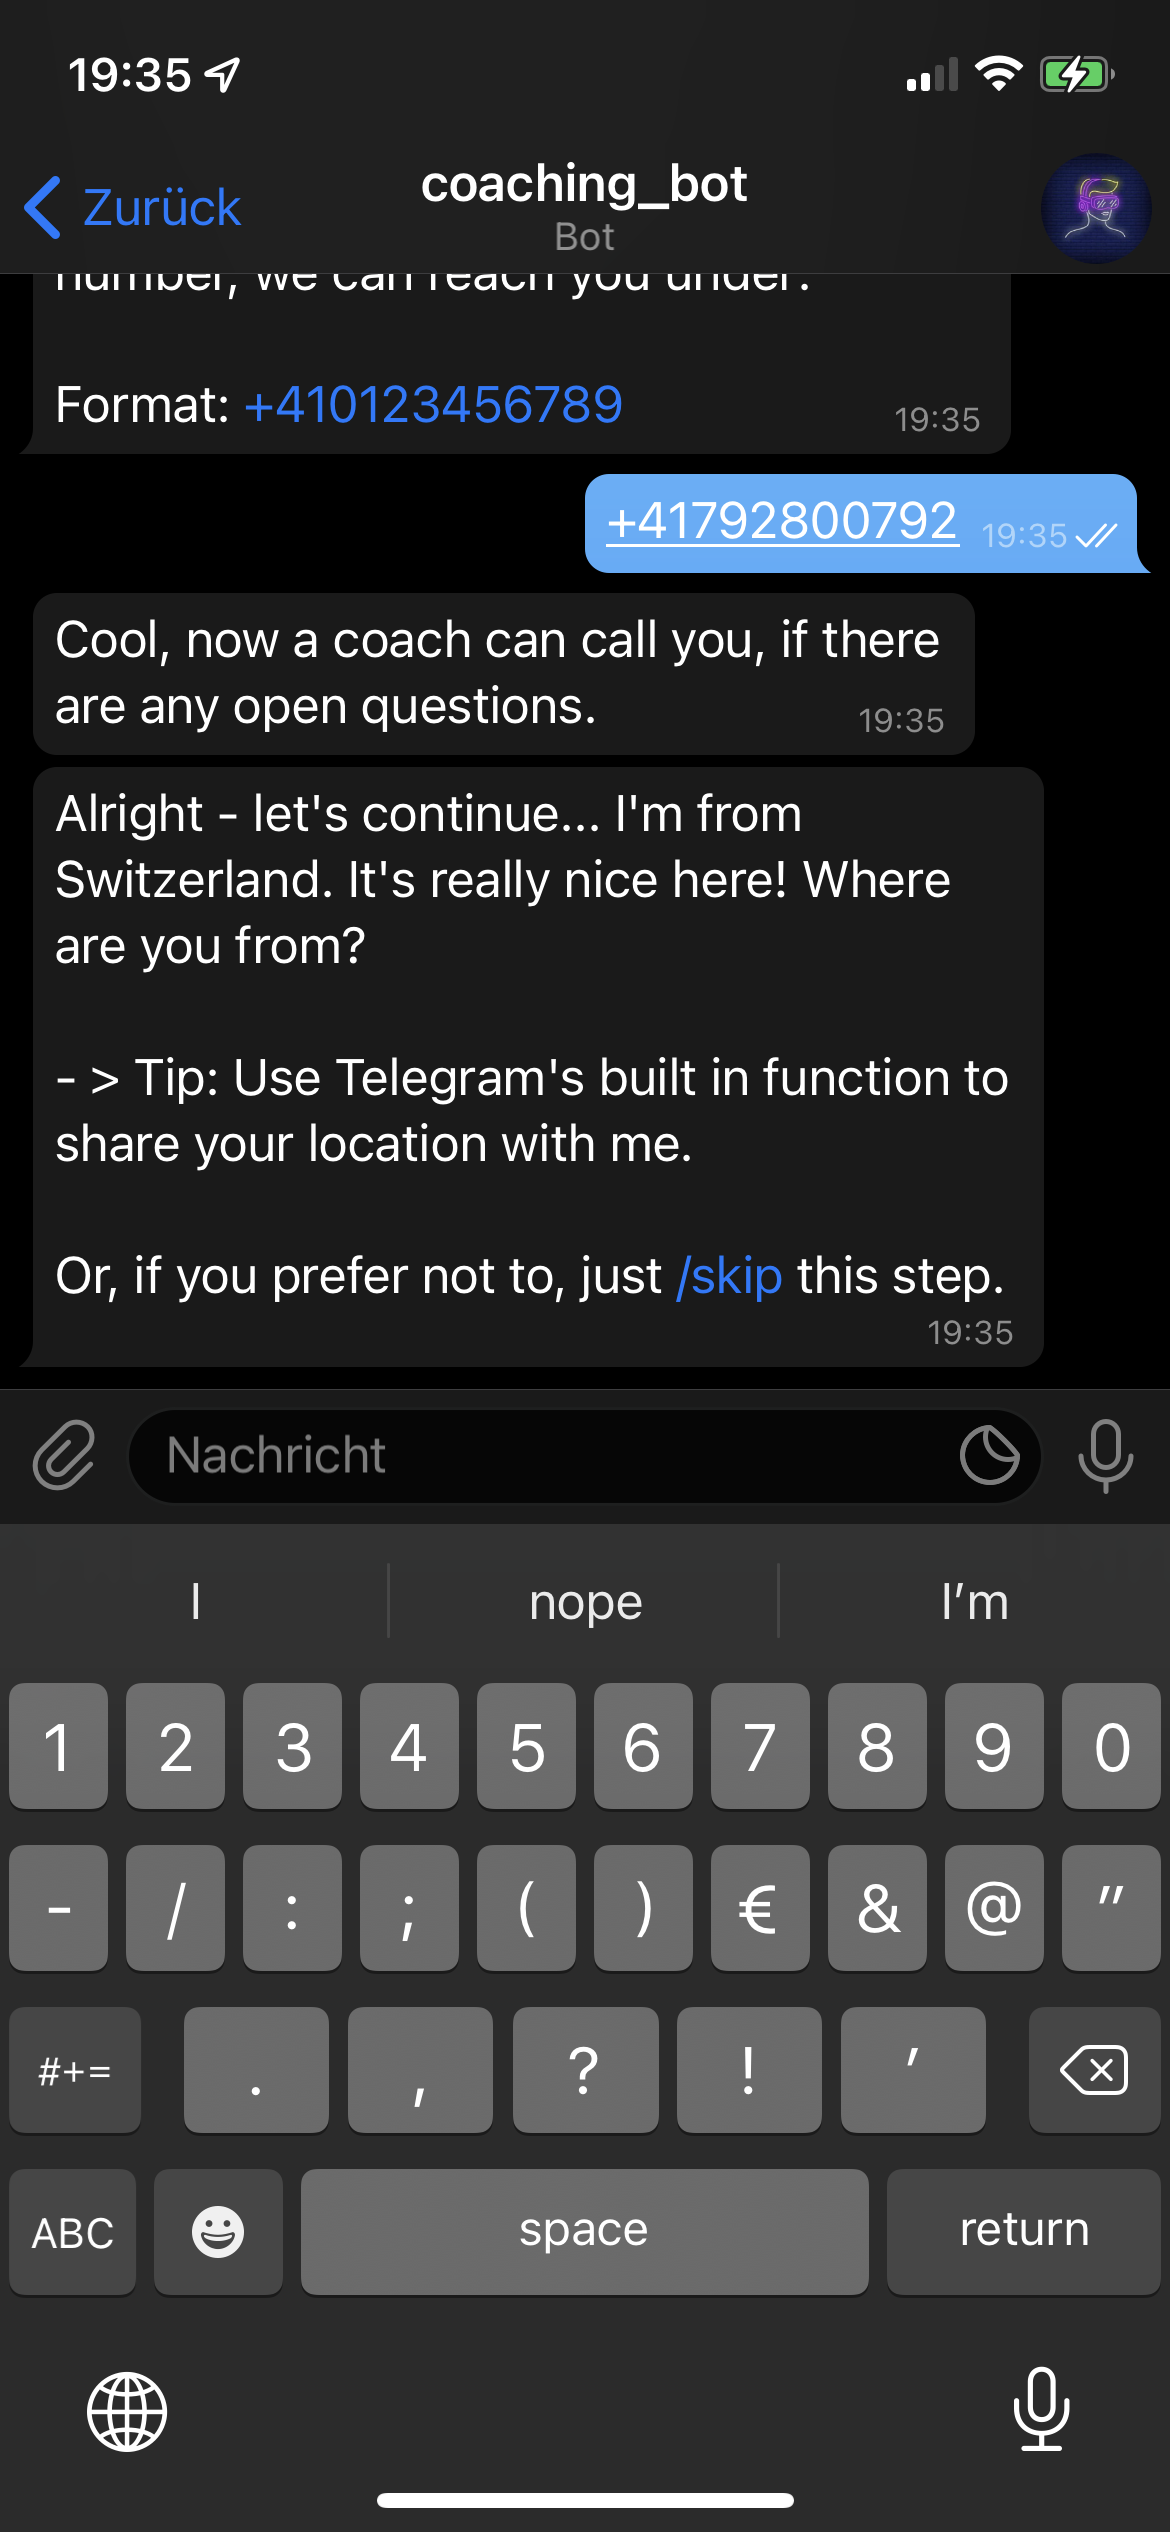
\includegraphics[width=\linewidth,height=300pt,keepaspectratio]{images/Screenshots/location.PNG}}
		
			\caption{Abfrage Telefonnummer und Standort}
		\end{minipage}
	\end{figure}


	% PAGE 03
	\begin{figure}
		\centering
		\begin{minipage}{.48\linewidth}
			\centering
			\subcaptionbox{Übergang zum Upload eines Fotos}
			{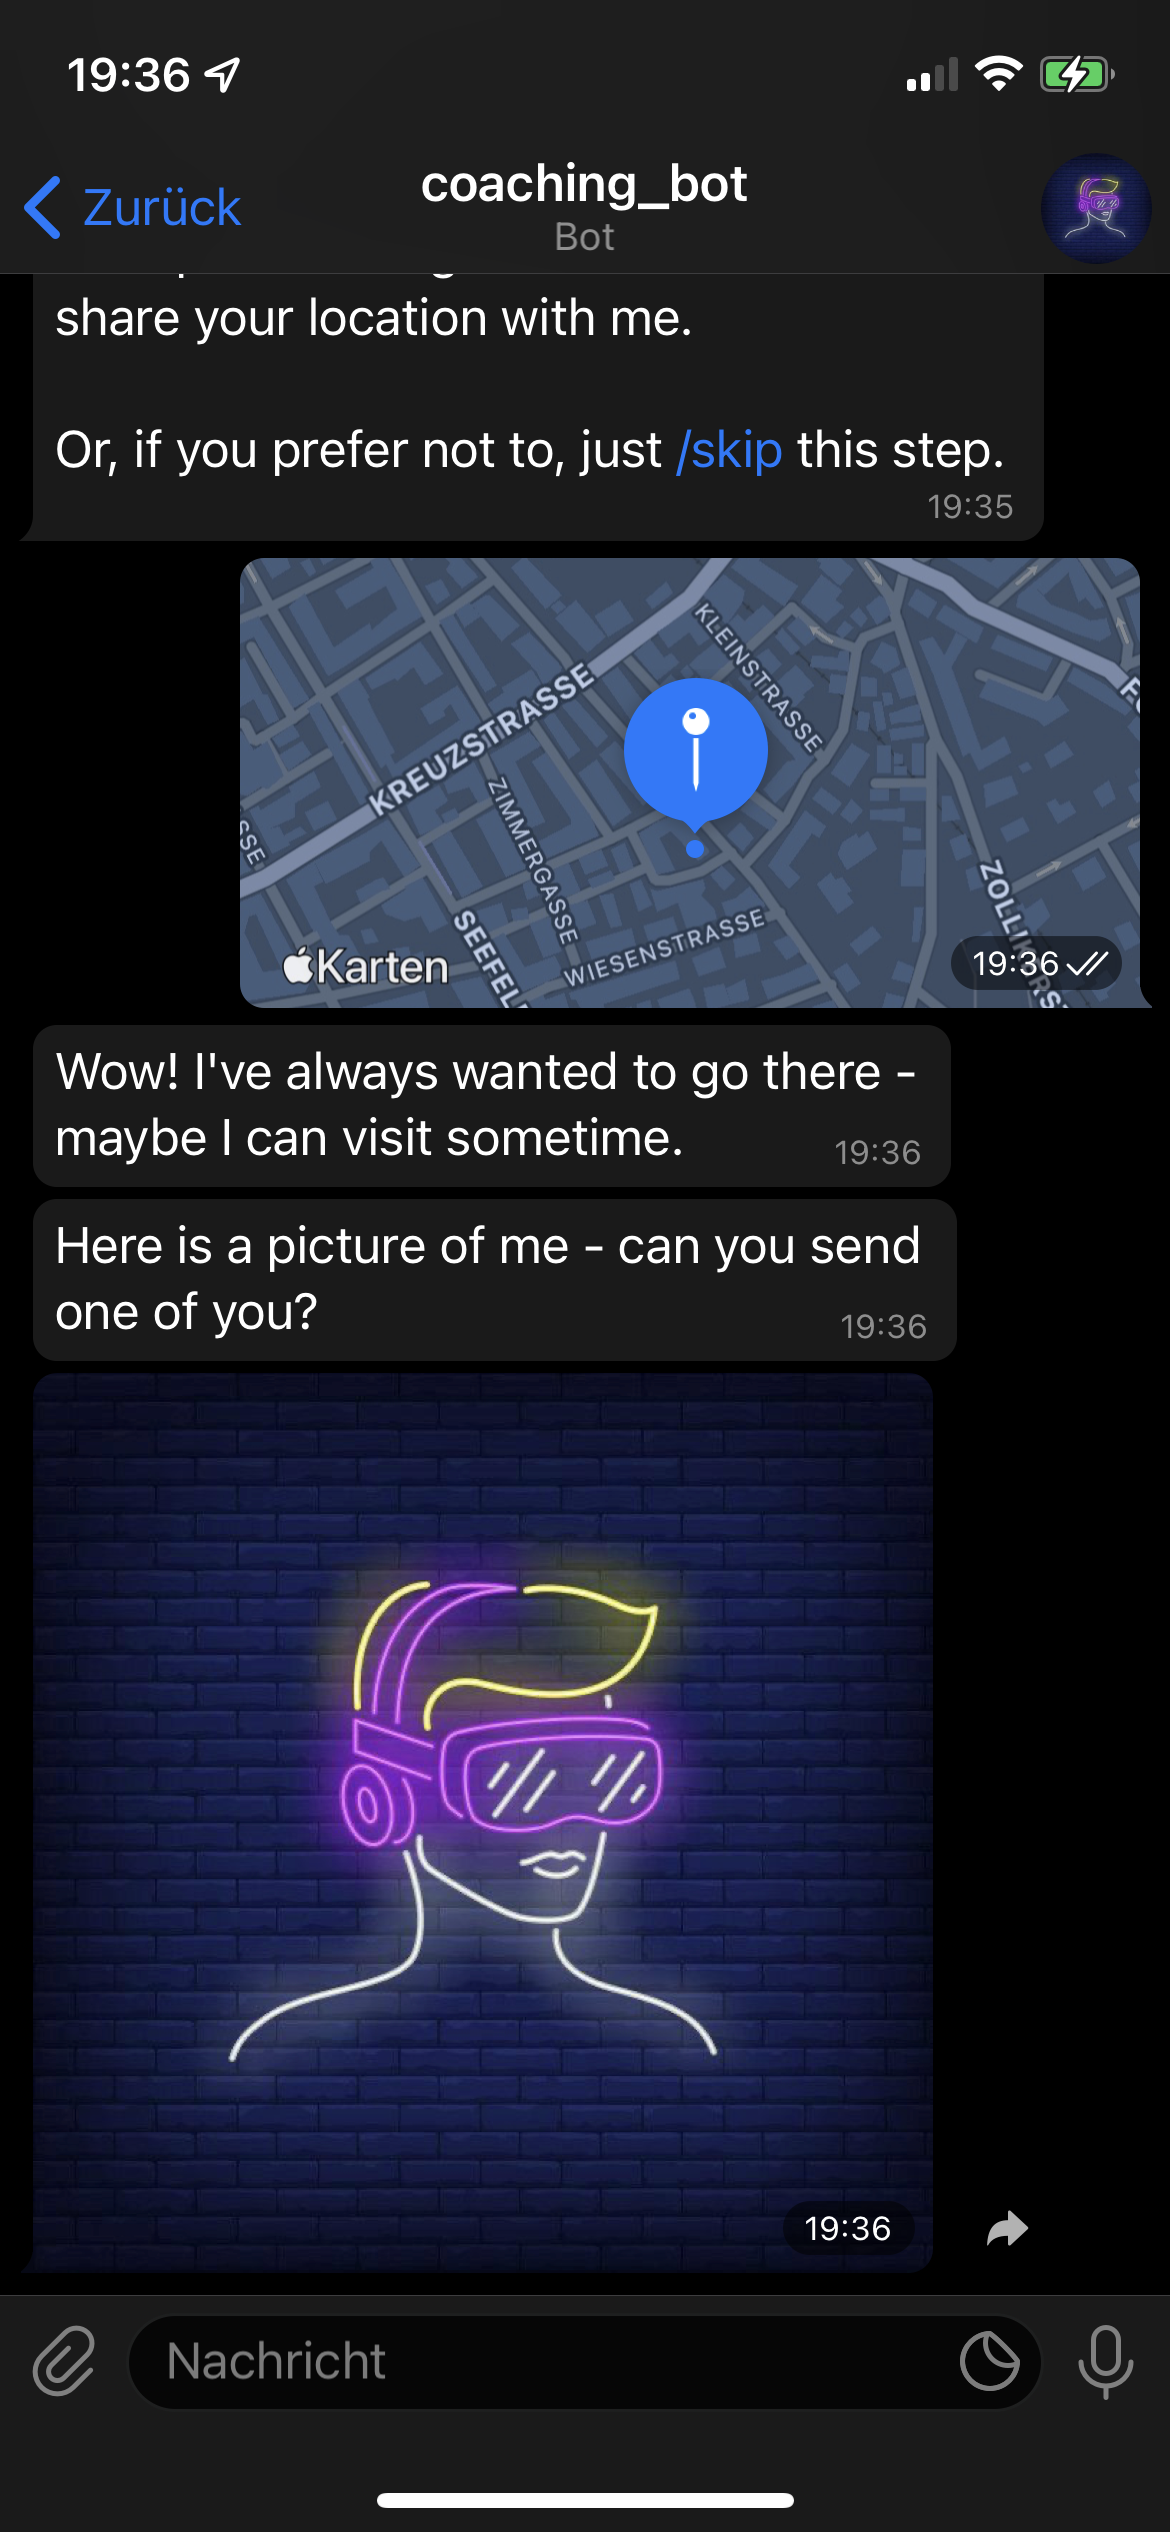
\includegraphics[width=\linewidth,height=300pt,keepaspectratio]{images/Screenshots/photo.PNG}}
		
			\subcaptionbox{Ende der Anmeldung und Übergang zur Terminauswahl}
			{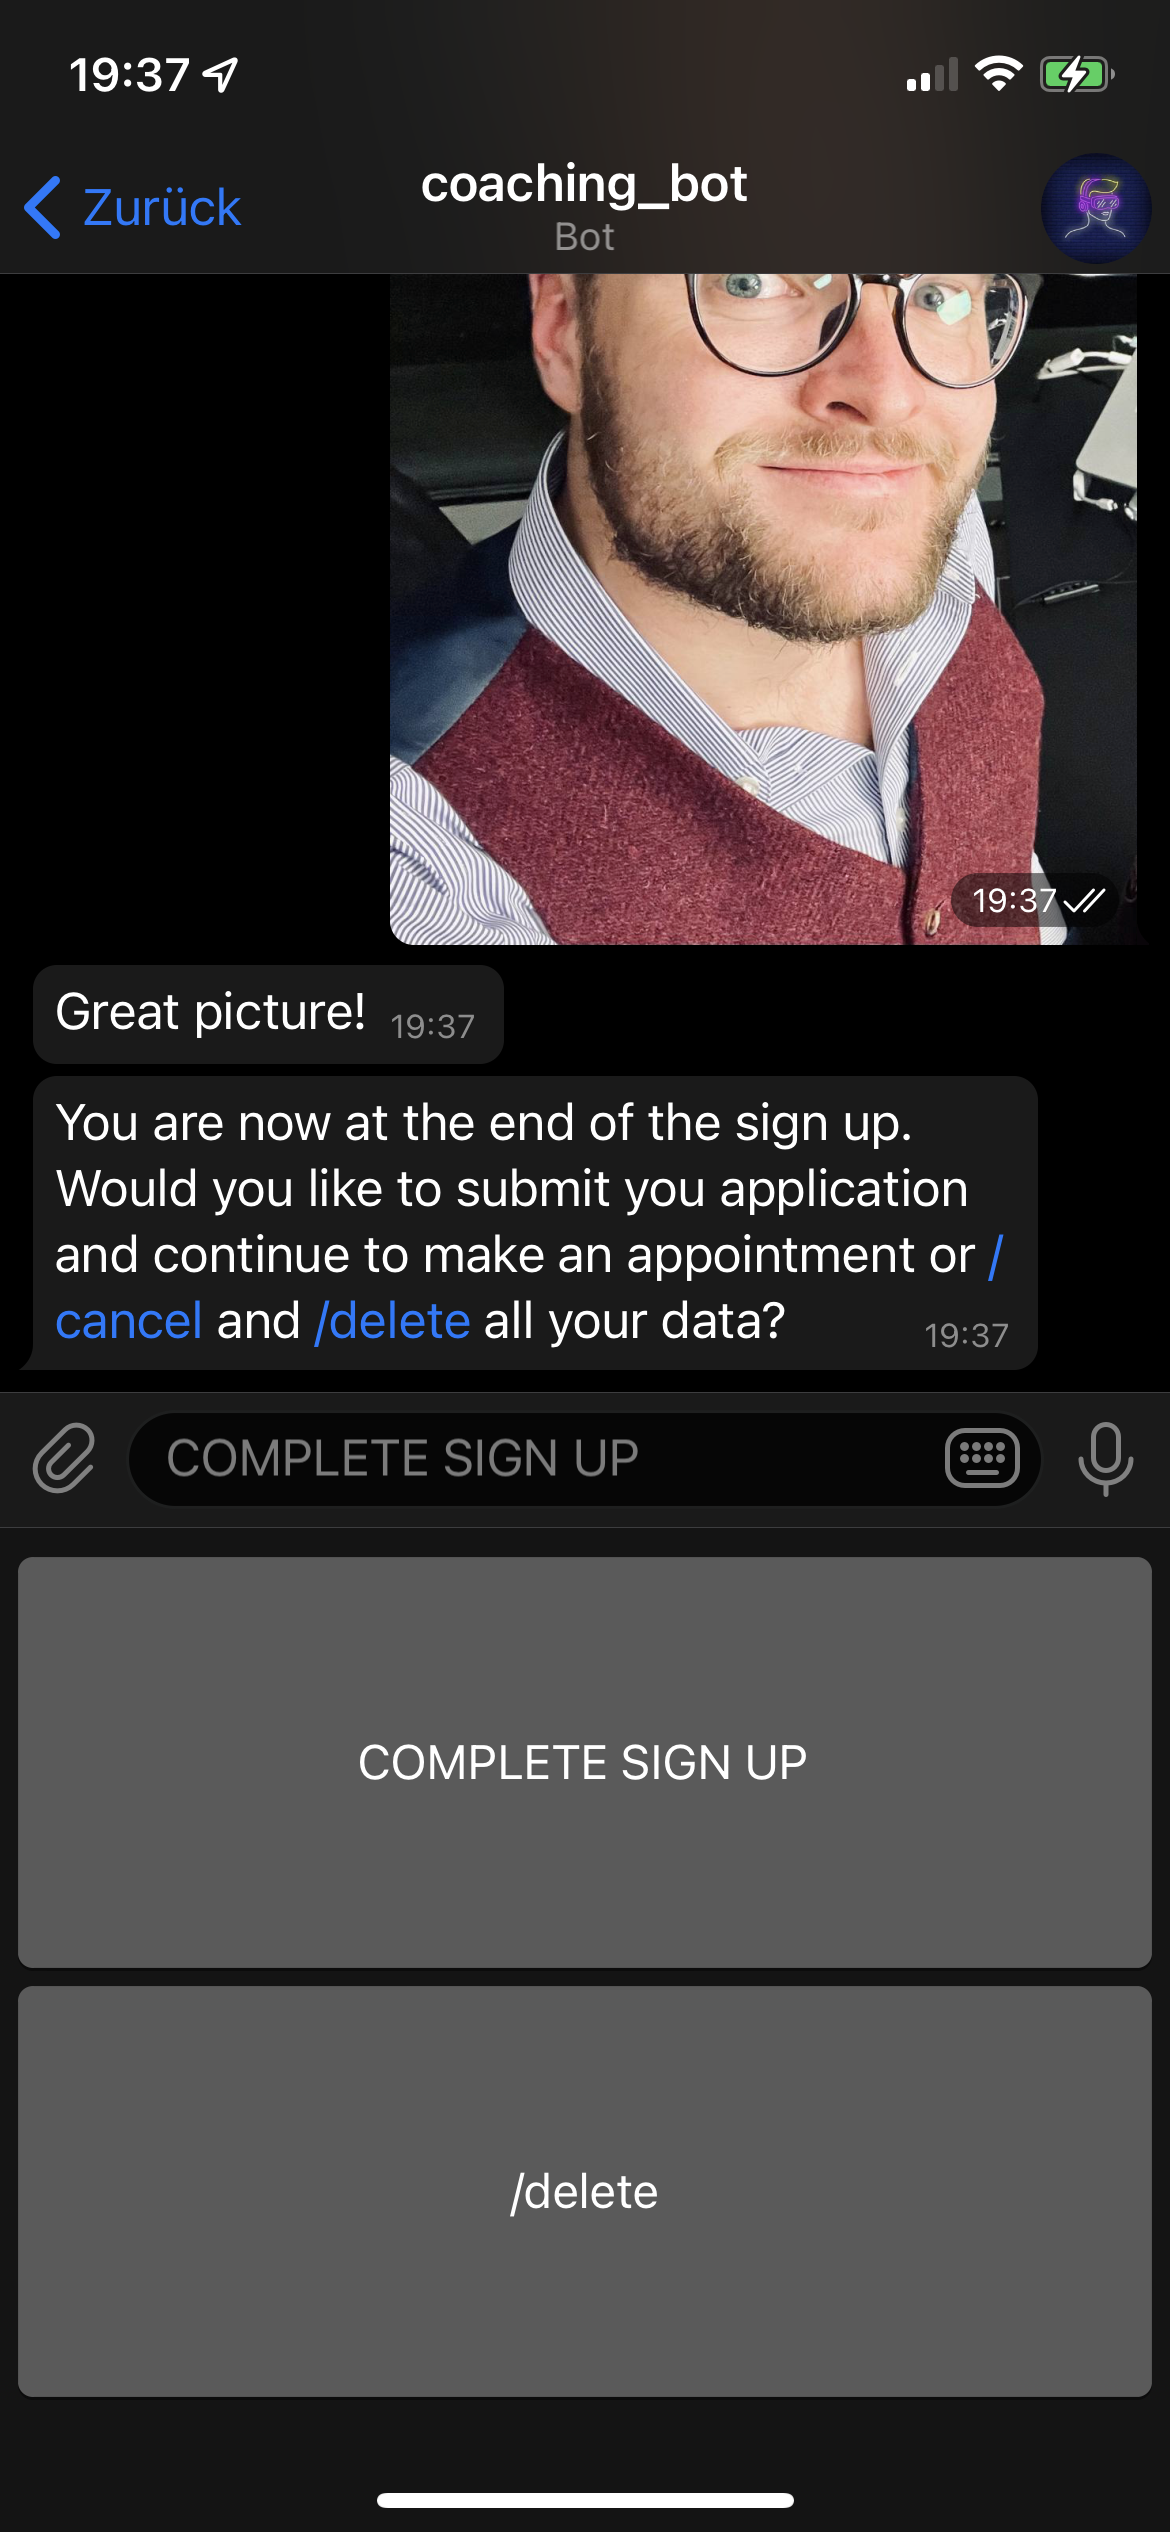
\includegraphics[width=\linewidth,height=300pt,keepaspectratio]{images/Screenshots/complete-sign-up.PNG}}
		
			\caption{Frage nach einem Bild des Nutzers und Abschluss des Sign-Ups}
		\end{minipage}\quad
		\begin{minipage}{.48\linewidth}
			\centering
			\subcaptionbox{Terminfindung}
			{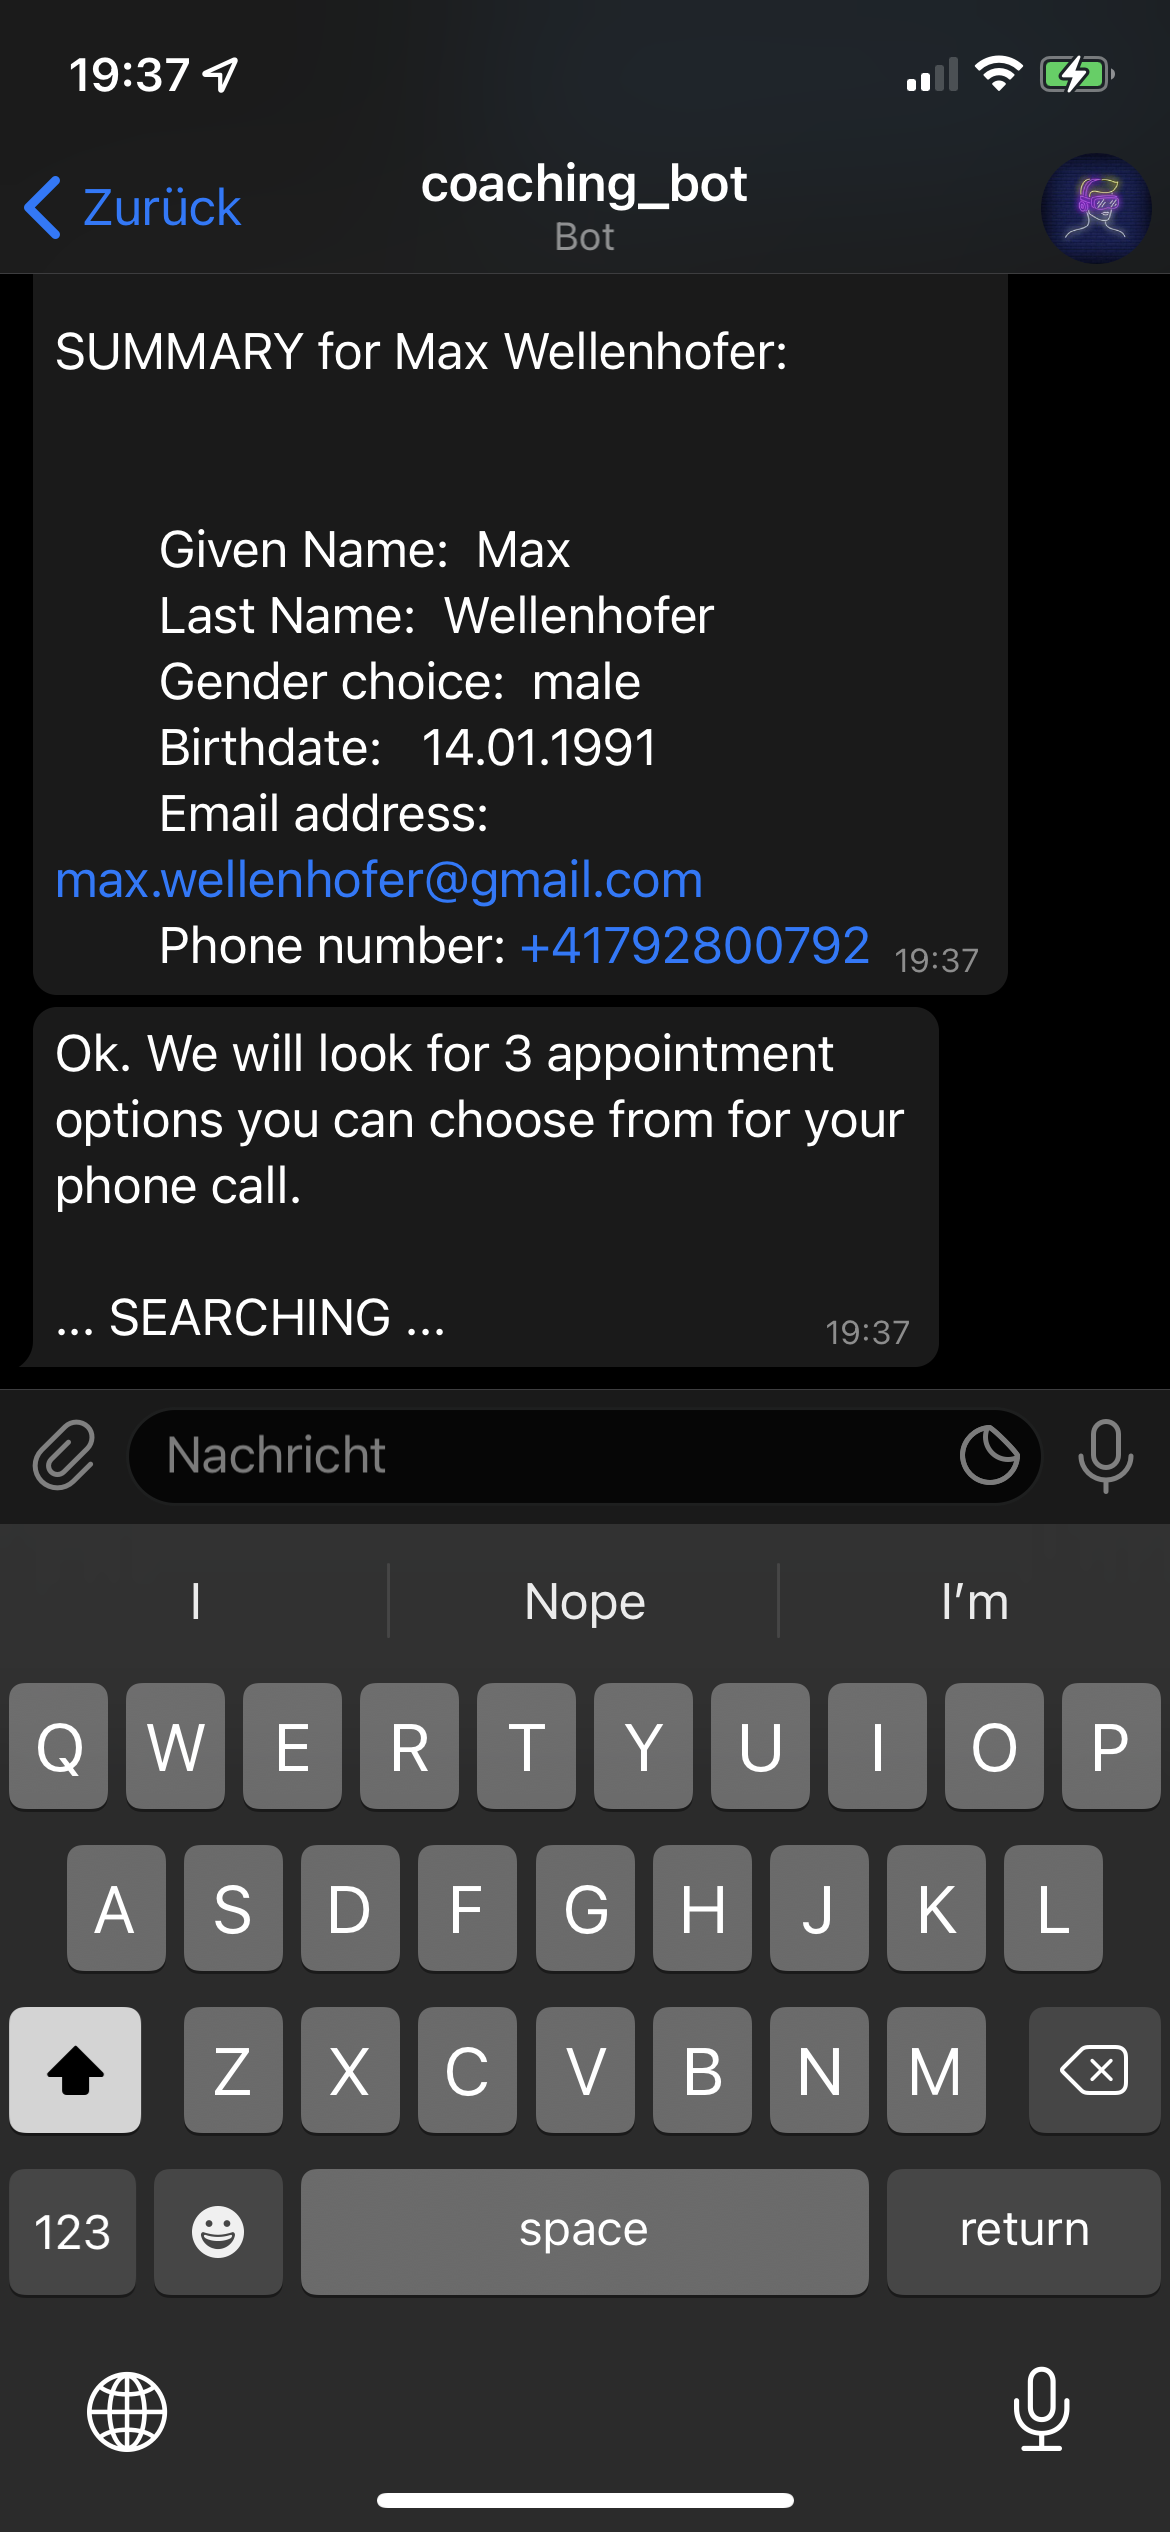
\includegraphics[width=\linewidth,height=300pt,keepaspectratio]{images/Screenshots/slot-search.PNG}}
		
			\subcaptionbox{Terminauswahl}
			{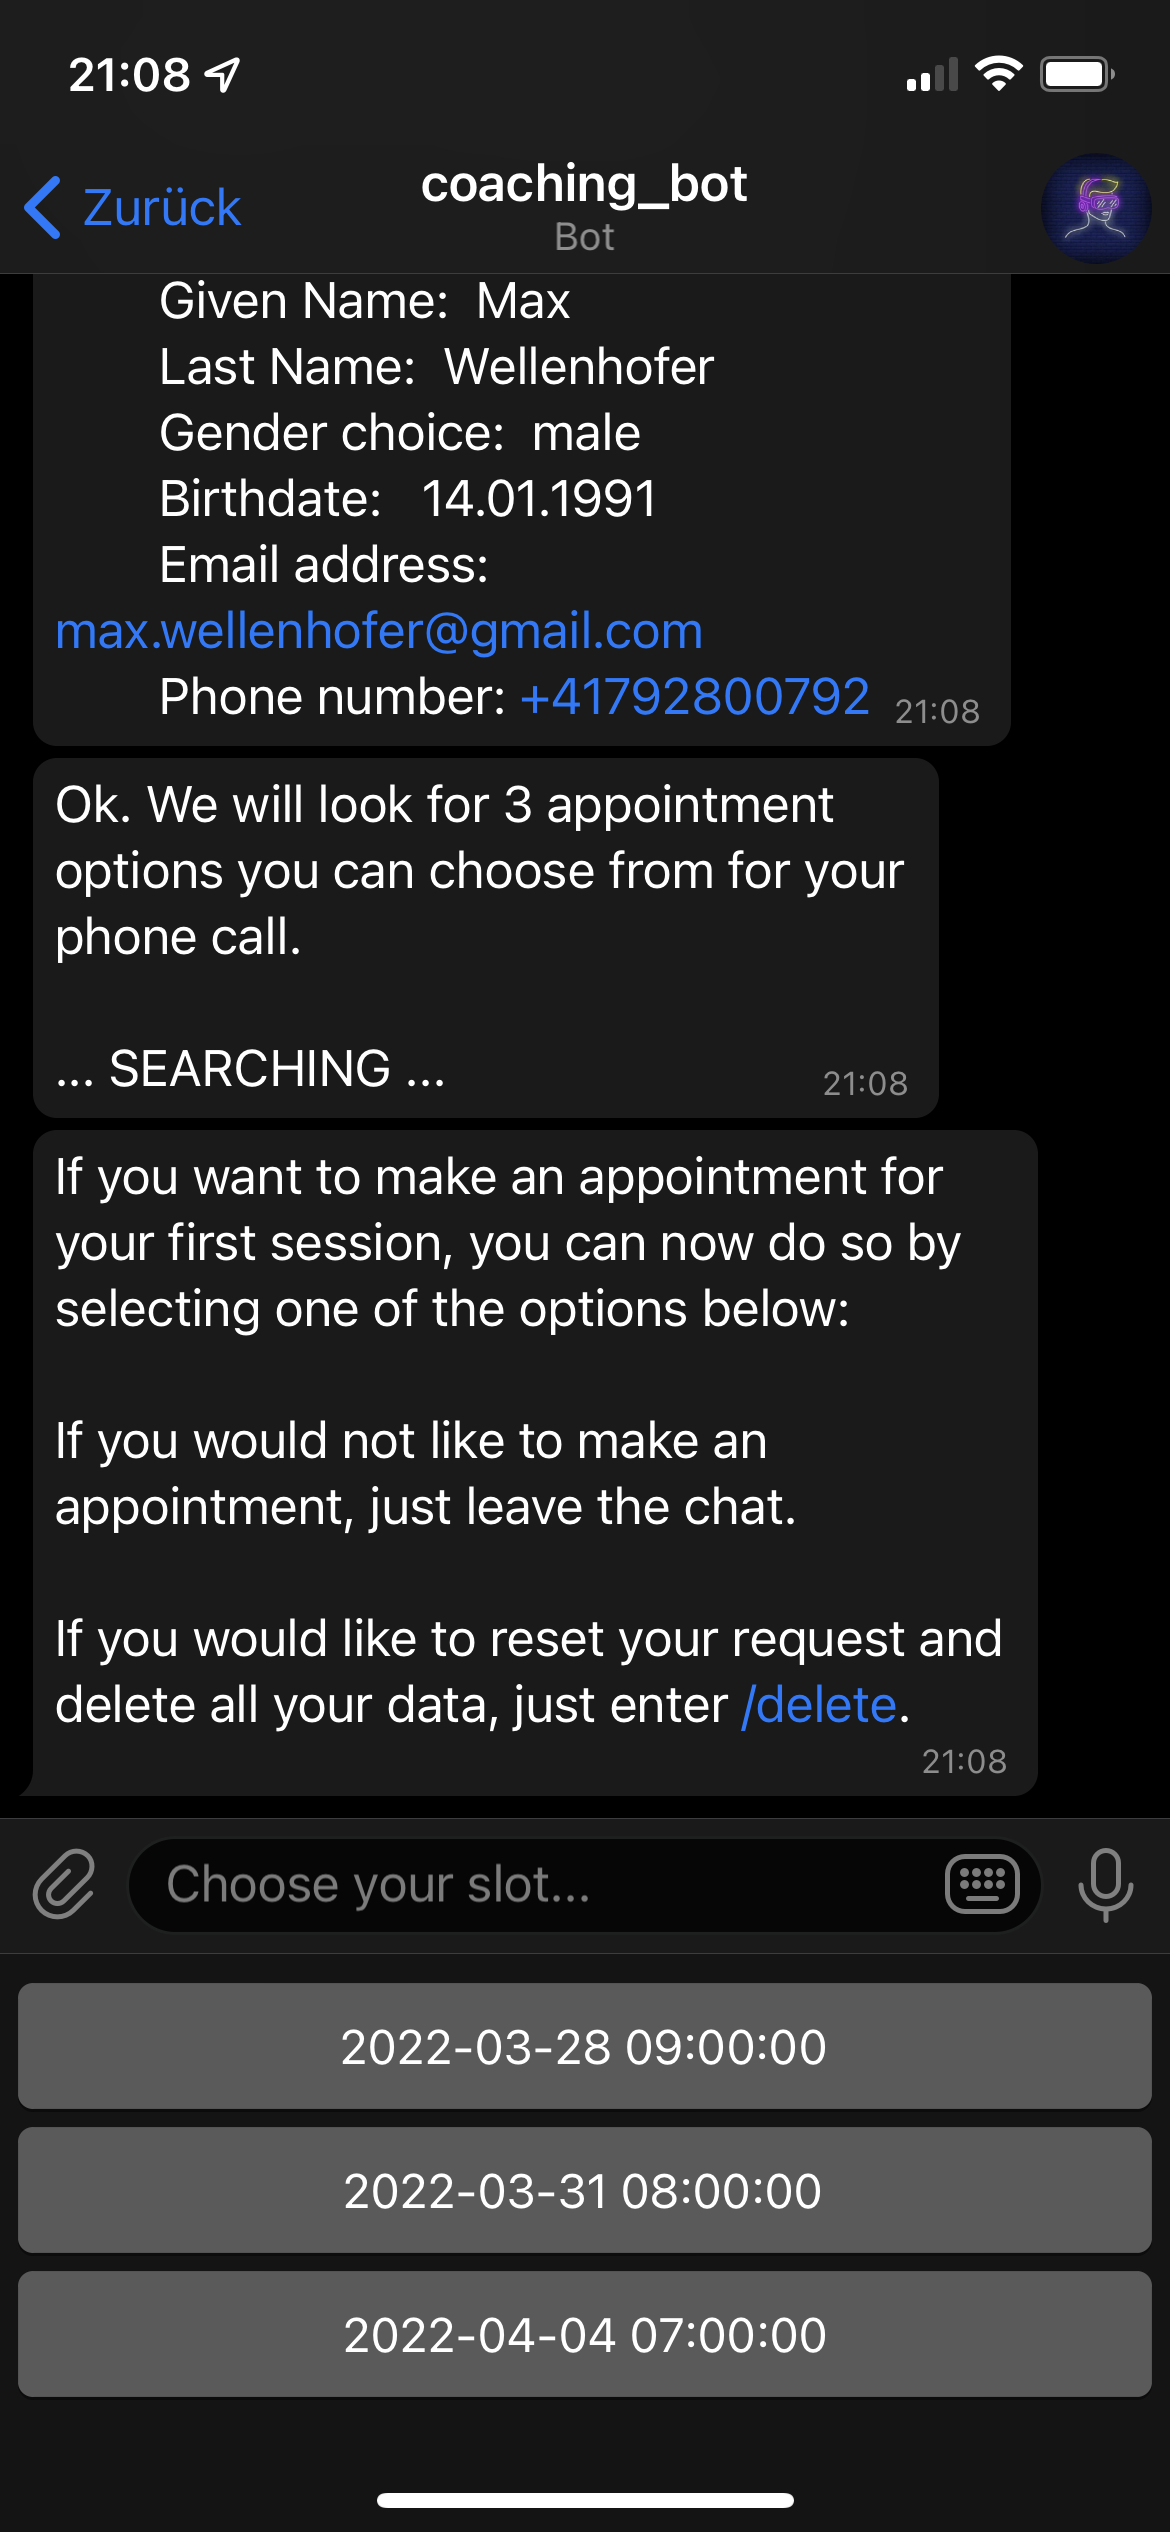
\includegraphics[width=\linewidth,height=300pt,keepaspectratio]{images/Screenshots/appointment-selection.PNG}}
		
			\caption{Terminsuche und -wahl}
		\end{minipage}
	\end{figure}


	% PAGE 04
	\begin{figure}
		\centering
		\begin{minipage}{.48\linewidth}
			\centering
			\subcaptionbox{Terminbestätigung}
			{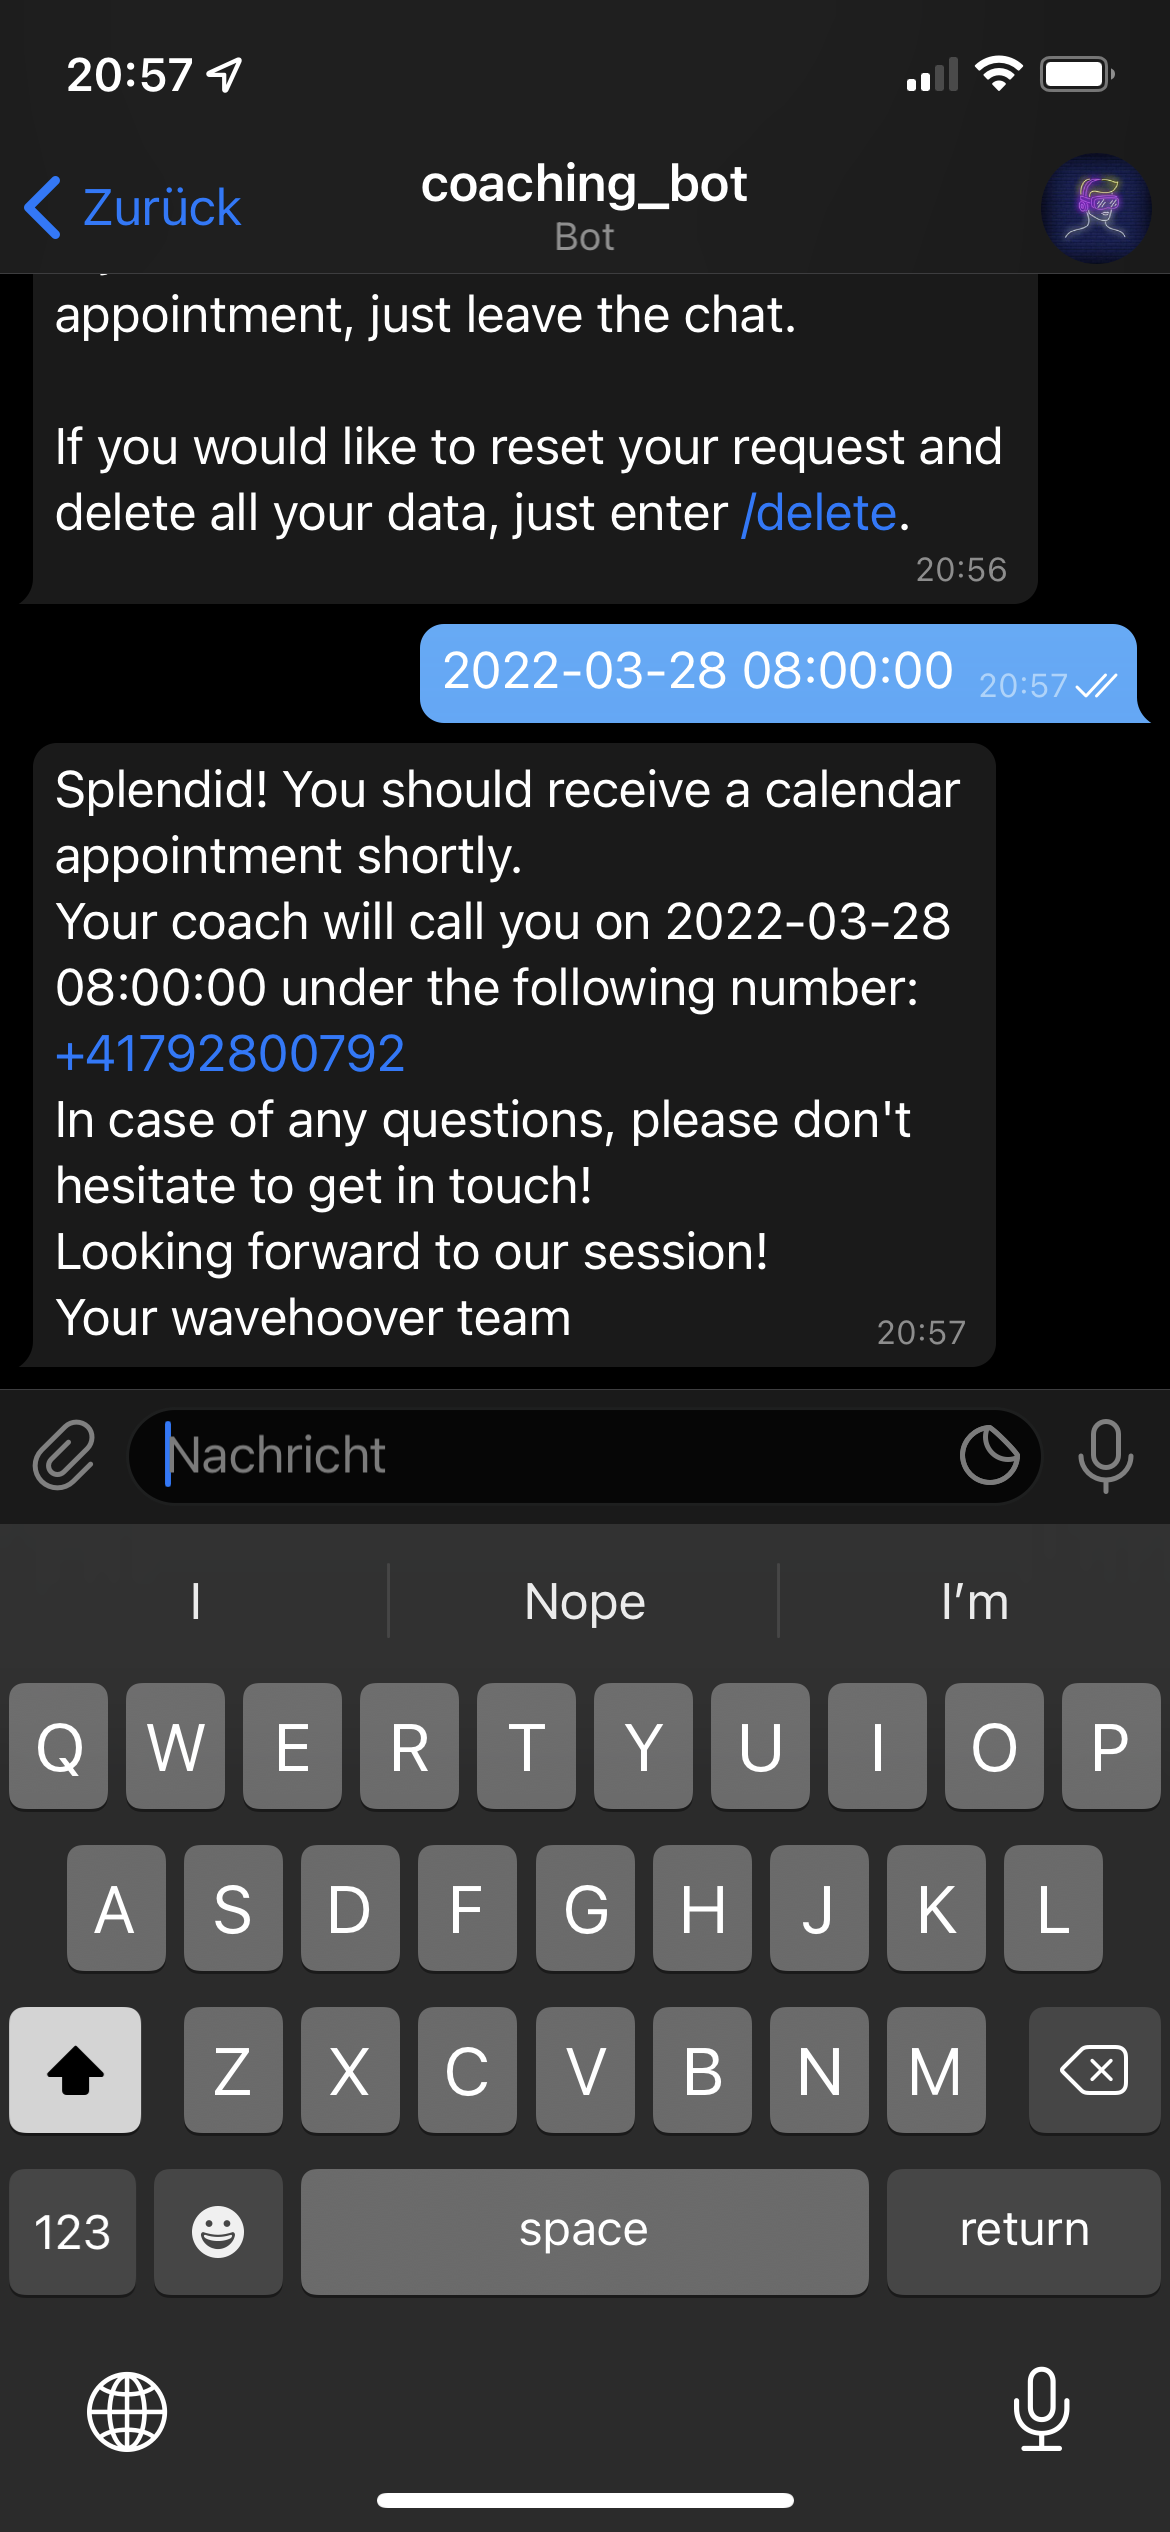
\includegraphics[width=\linewidth,height=300pt,keepaspectratio]{images/Screenshots/appointment-made.PNG}}
		
			\subcaptionbox{Kalendereinladung}
			{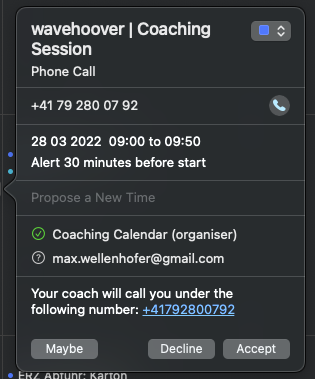
\includegraphics[width=\linewidth,height=300pt,keepaspectratio]{images/Screenshots/calendar-invite.png}}
		
			\caption{Bestätigung, dass Termin vereinbart wurde und die entsprechende Bestätigung per Kalender-Client}
		\end{minipage}\quad
		\begin{minipage}{.48\linewidth}
			\centering
			\subcaptionbox{Rückkehr zum Bot, wenn bereits ein Termin vereinbart wurde}
			{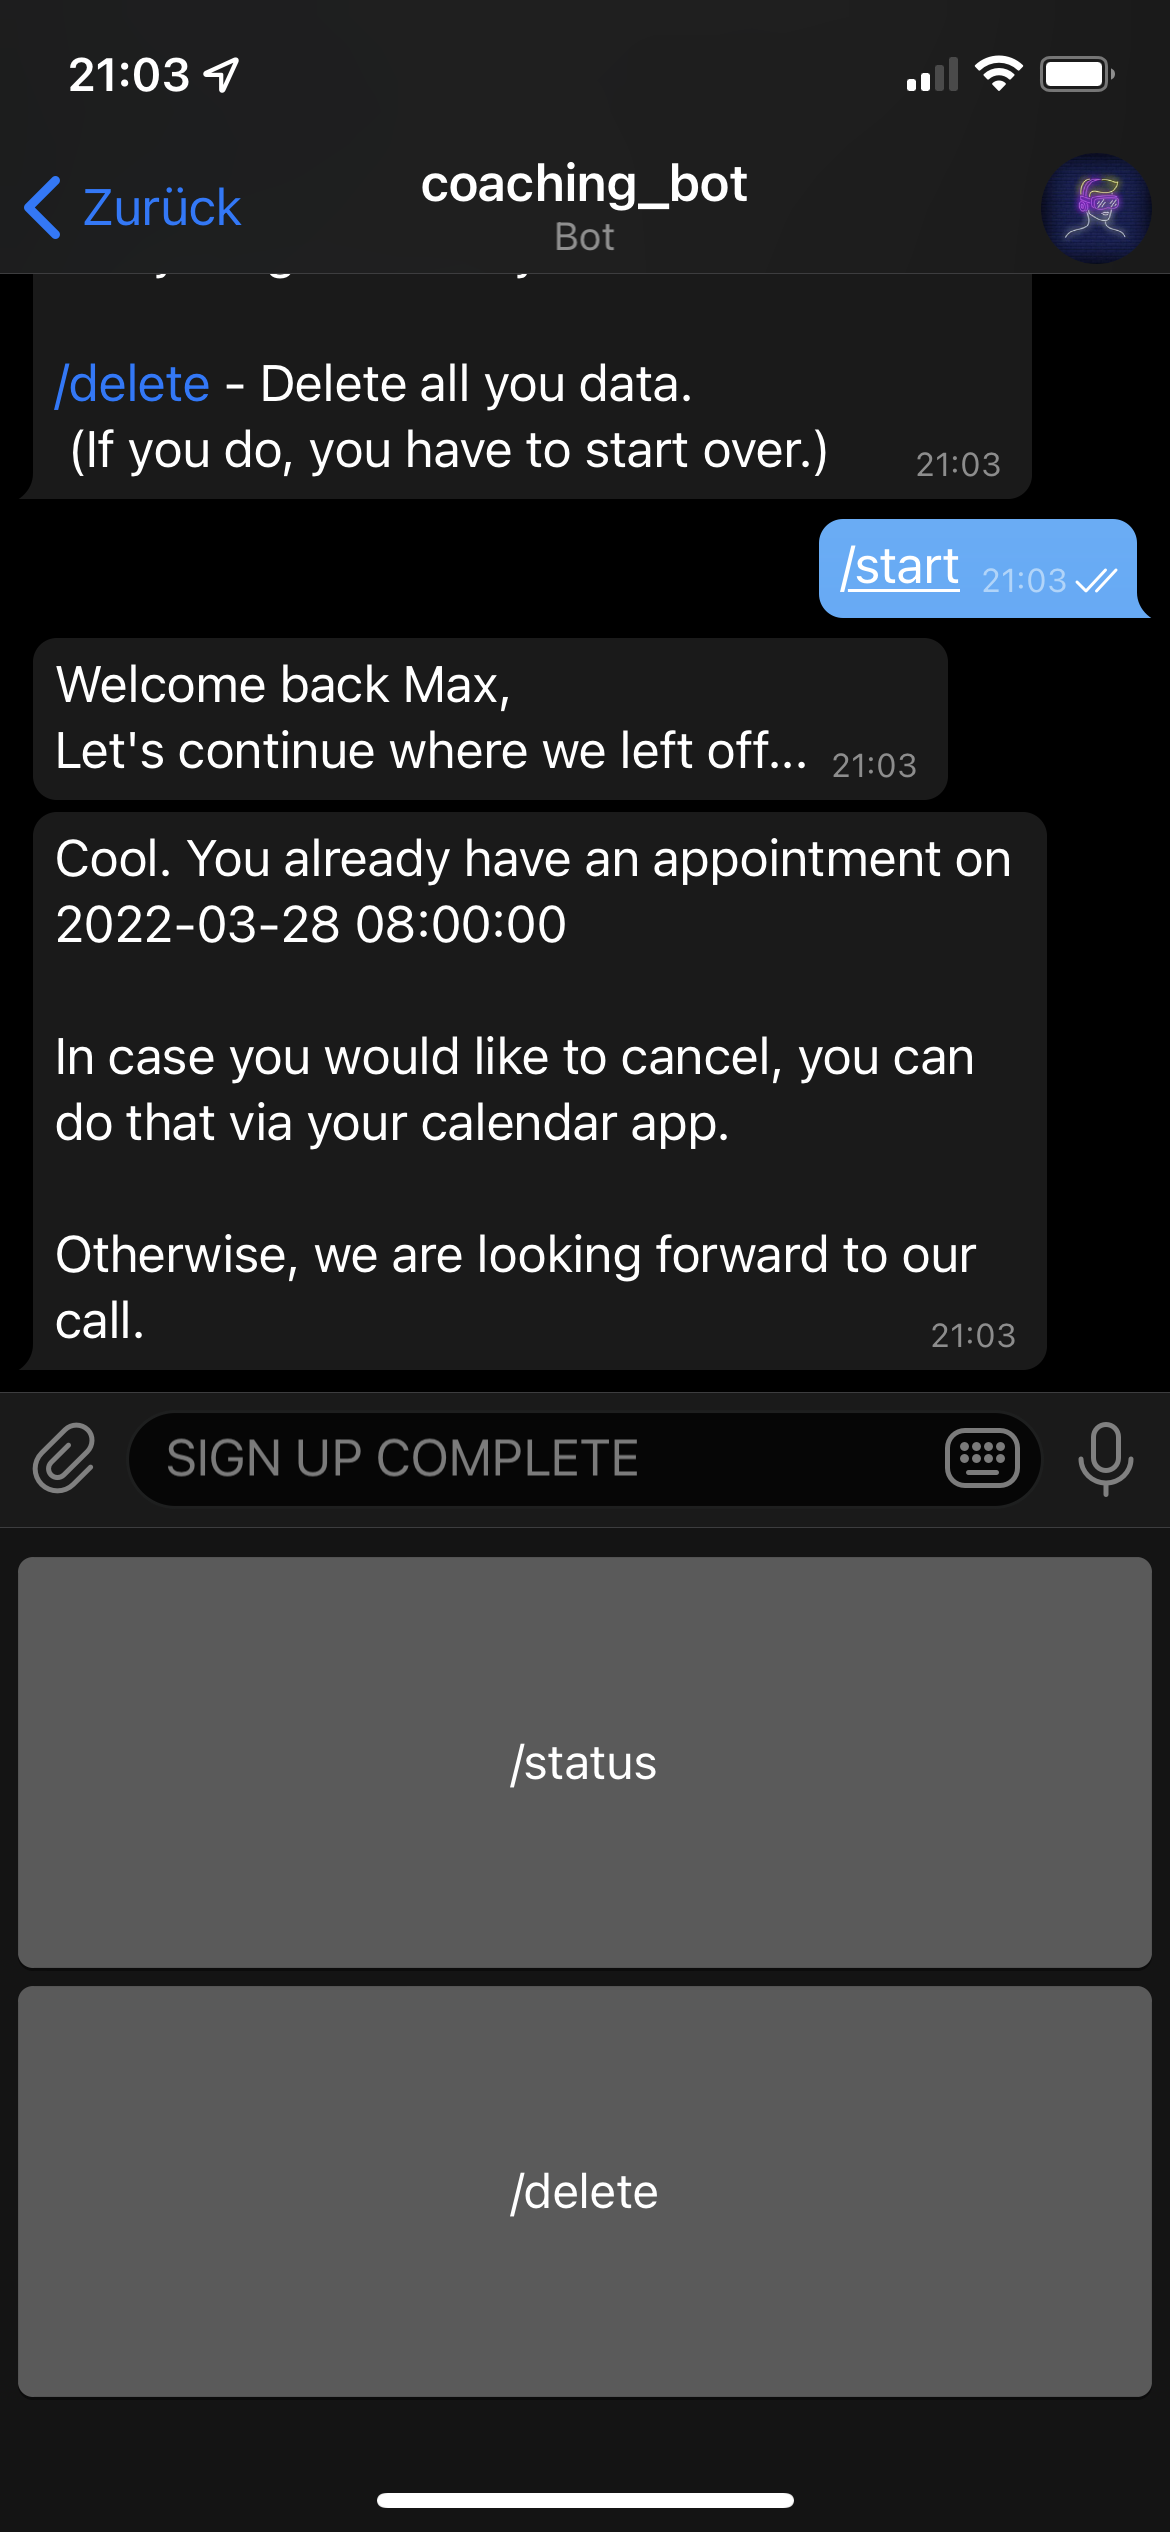
\includegraphics[width=\linewidth,height=300pt,keepaspectratio]{images/Screenshots/return-with-appointment.PNG}}
		
			\subcaptionbox{Statusabfrage und Hilfe}
			{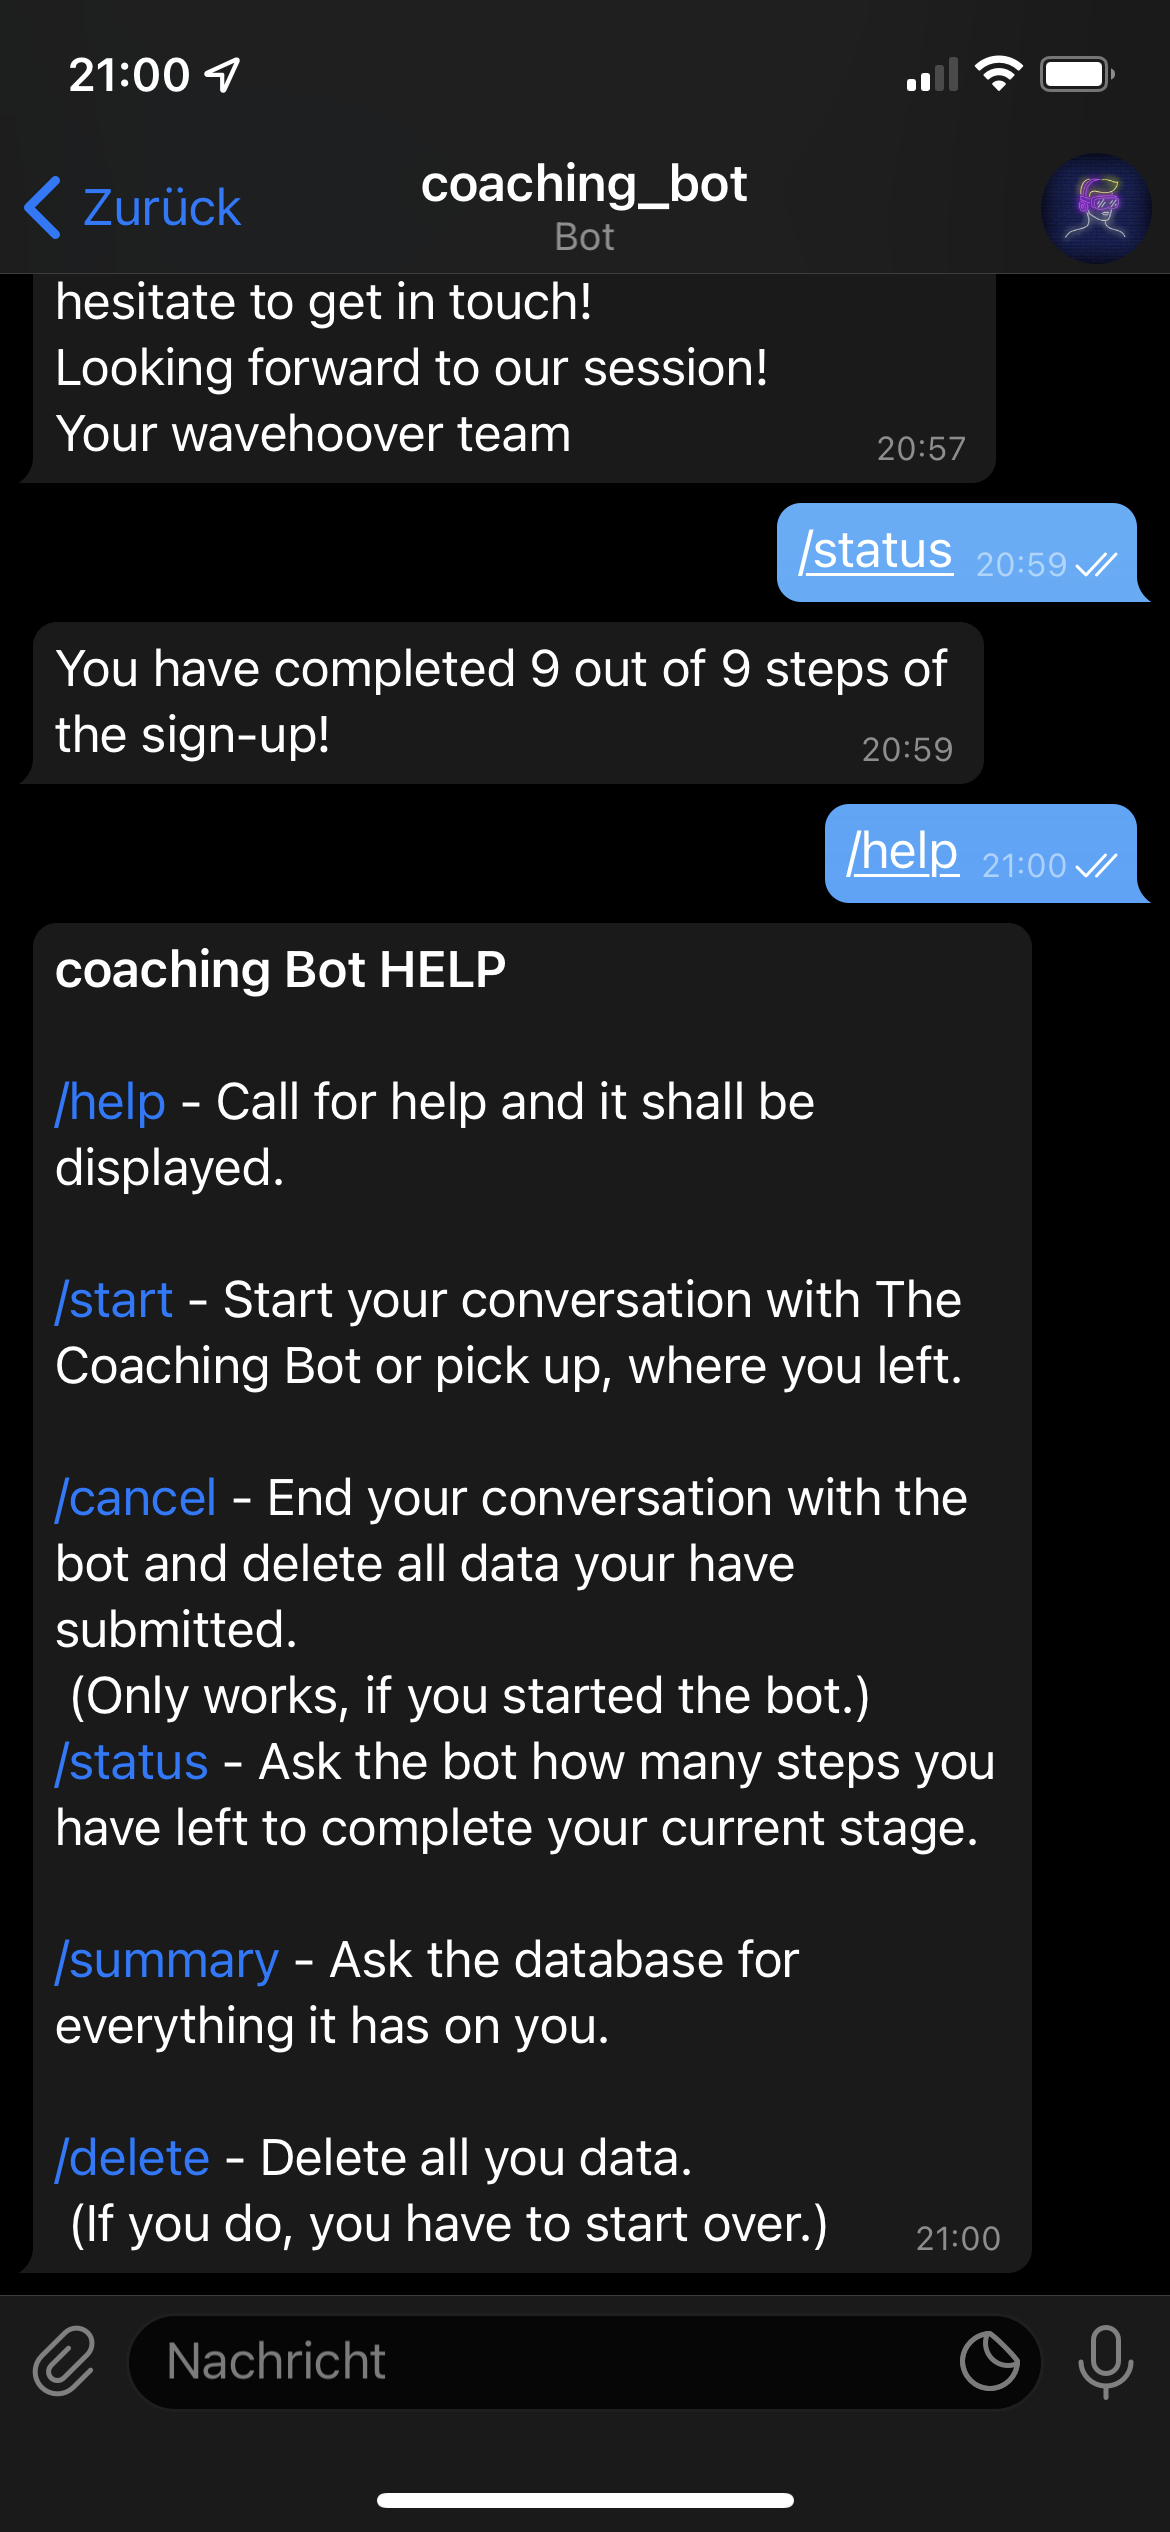
\includegraphics[width=\linewidth,height=300pt,keepaspectratio]{images/Screenshots/status-and-help.PNG}}
		
			\caption{Rückkehr des Nutzers nach Beendigung des Konversationsflusses und Ausgabe Meta-Funktionen}
		\end{minipage}
	\end{figure}


	% PAGE 05
	\begin{figure}
		\centering
		\begin{minipage}{.48\linewidth}
			\centering
			\subcaptionbox{Nutzerdaten löschen und Neustart des Bots}
			{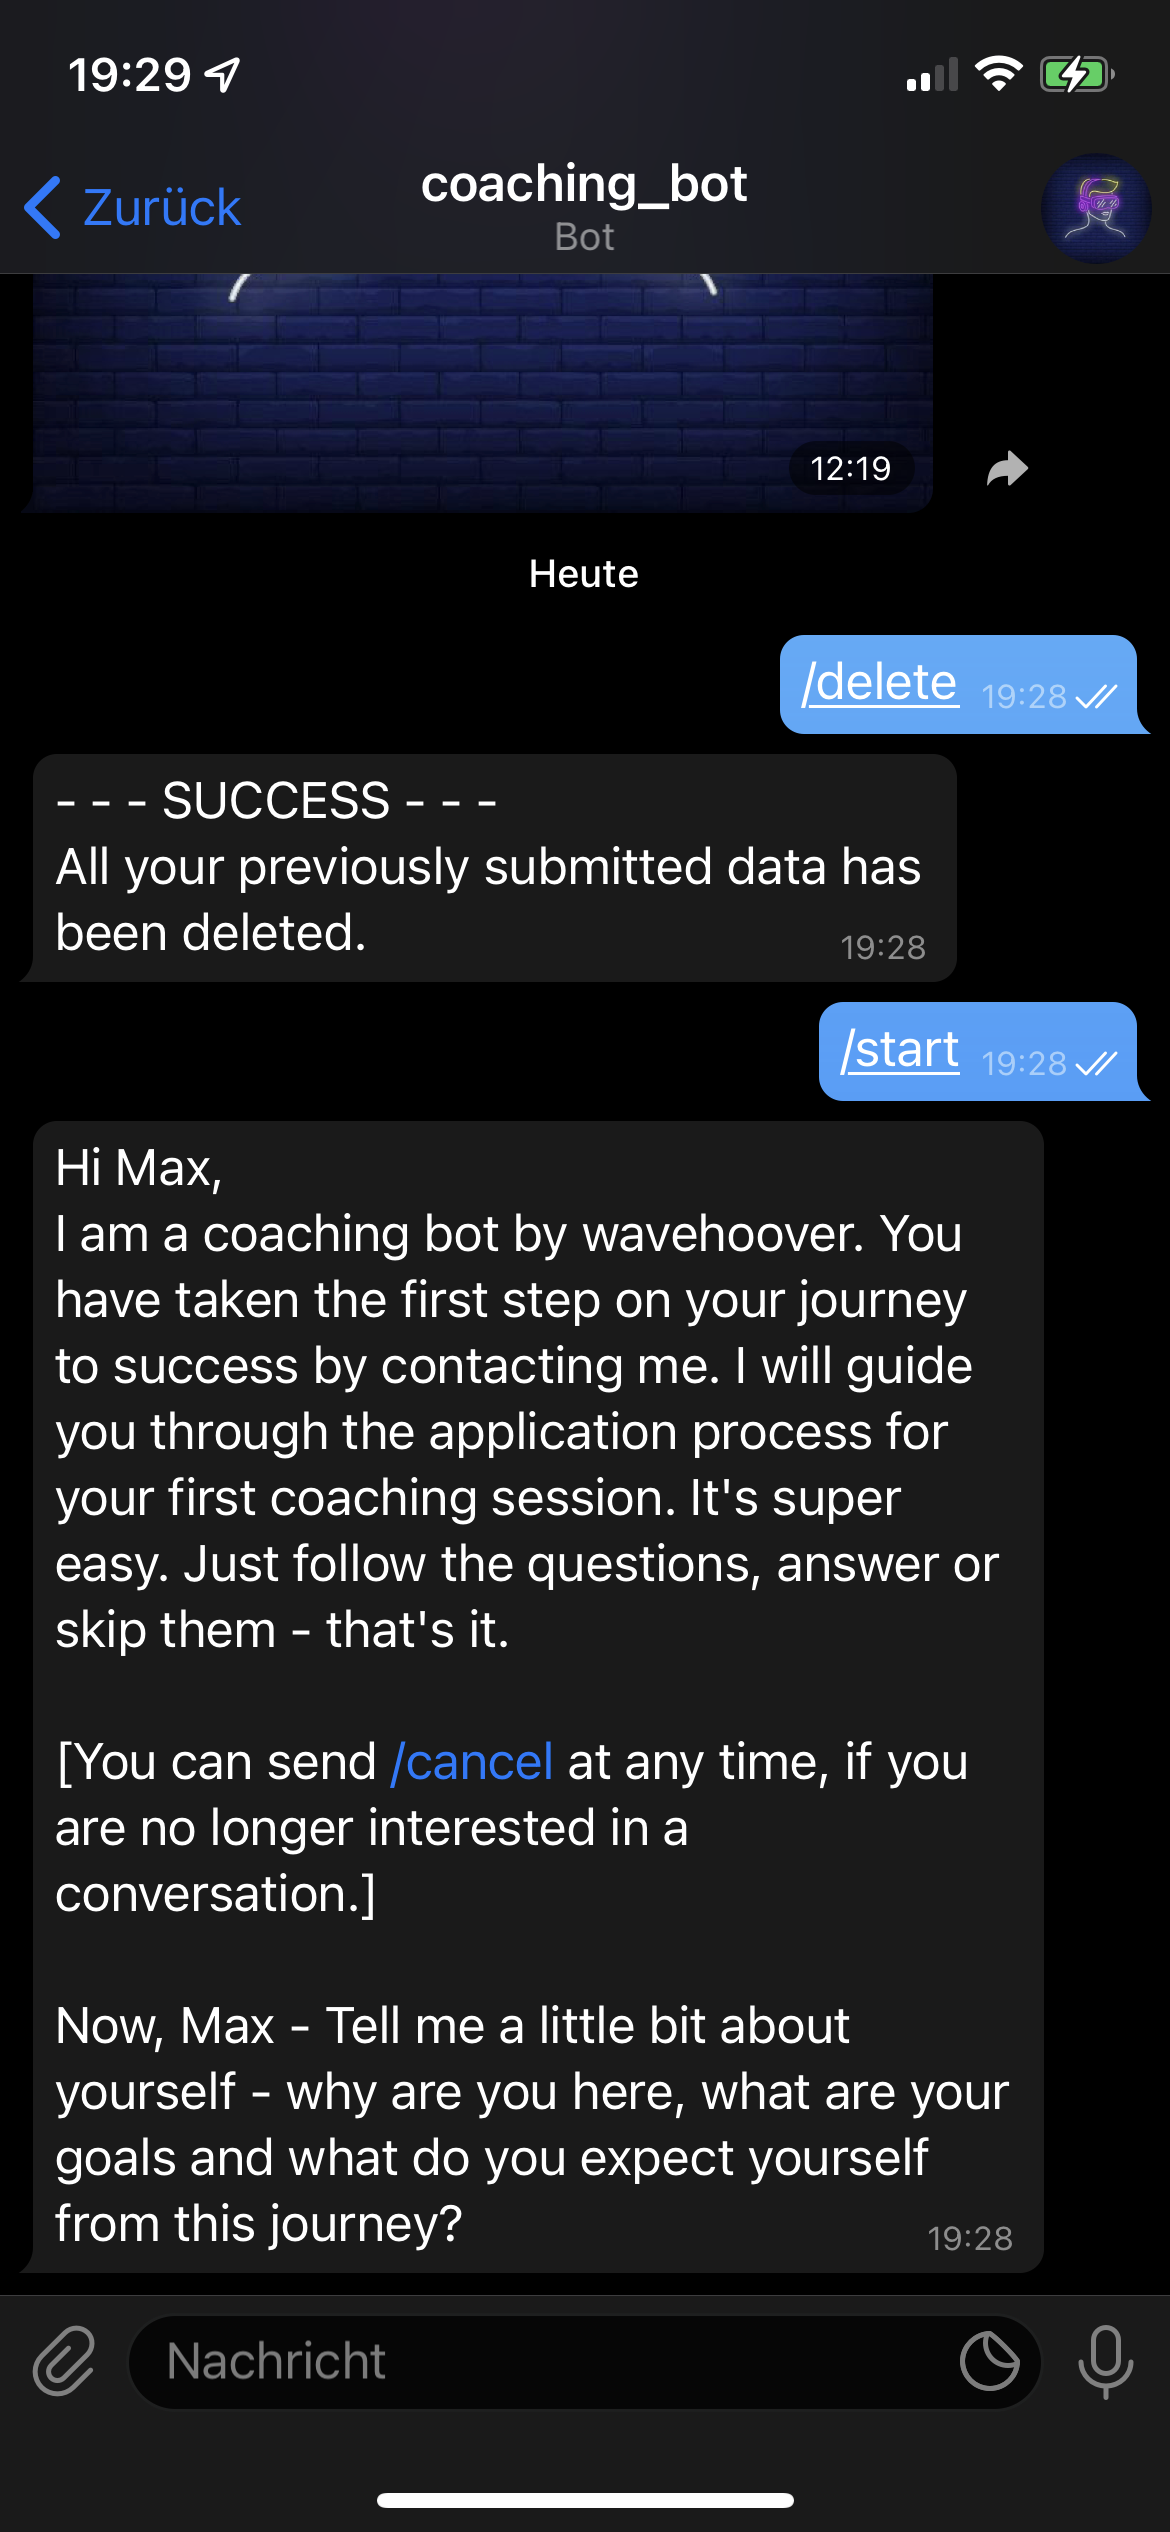
\includegraphics[width=\linewidth,height=300pt,keepaspectratio]{images/Screenshots/delete-and-restart.PNG}}
		
			\caption{Resultat aus \/delte und \/start}
		\end{minipage}\quad
	\end{figure}


	\begin{figure}
		\centering
		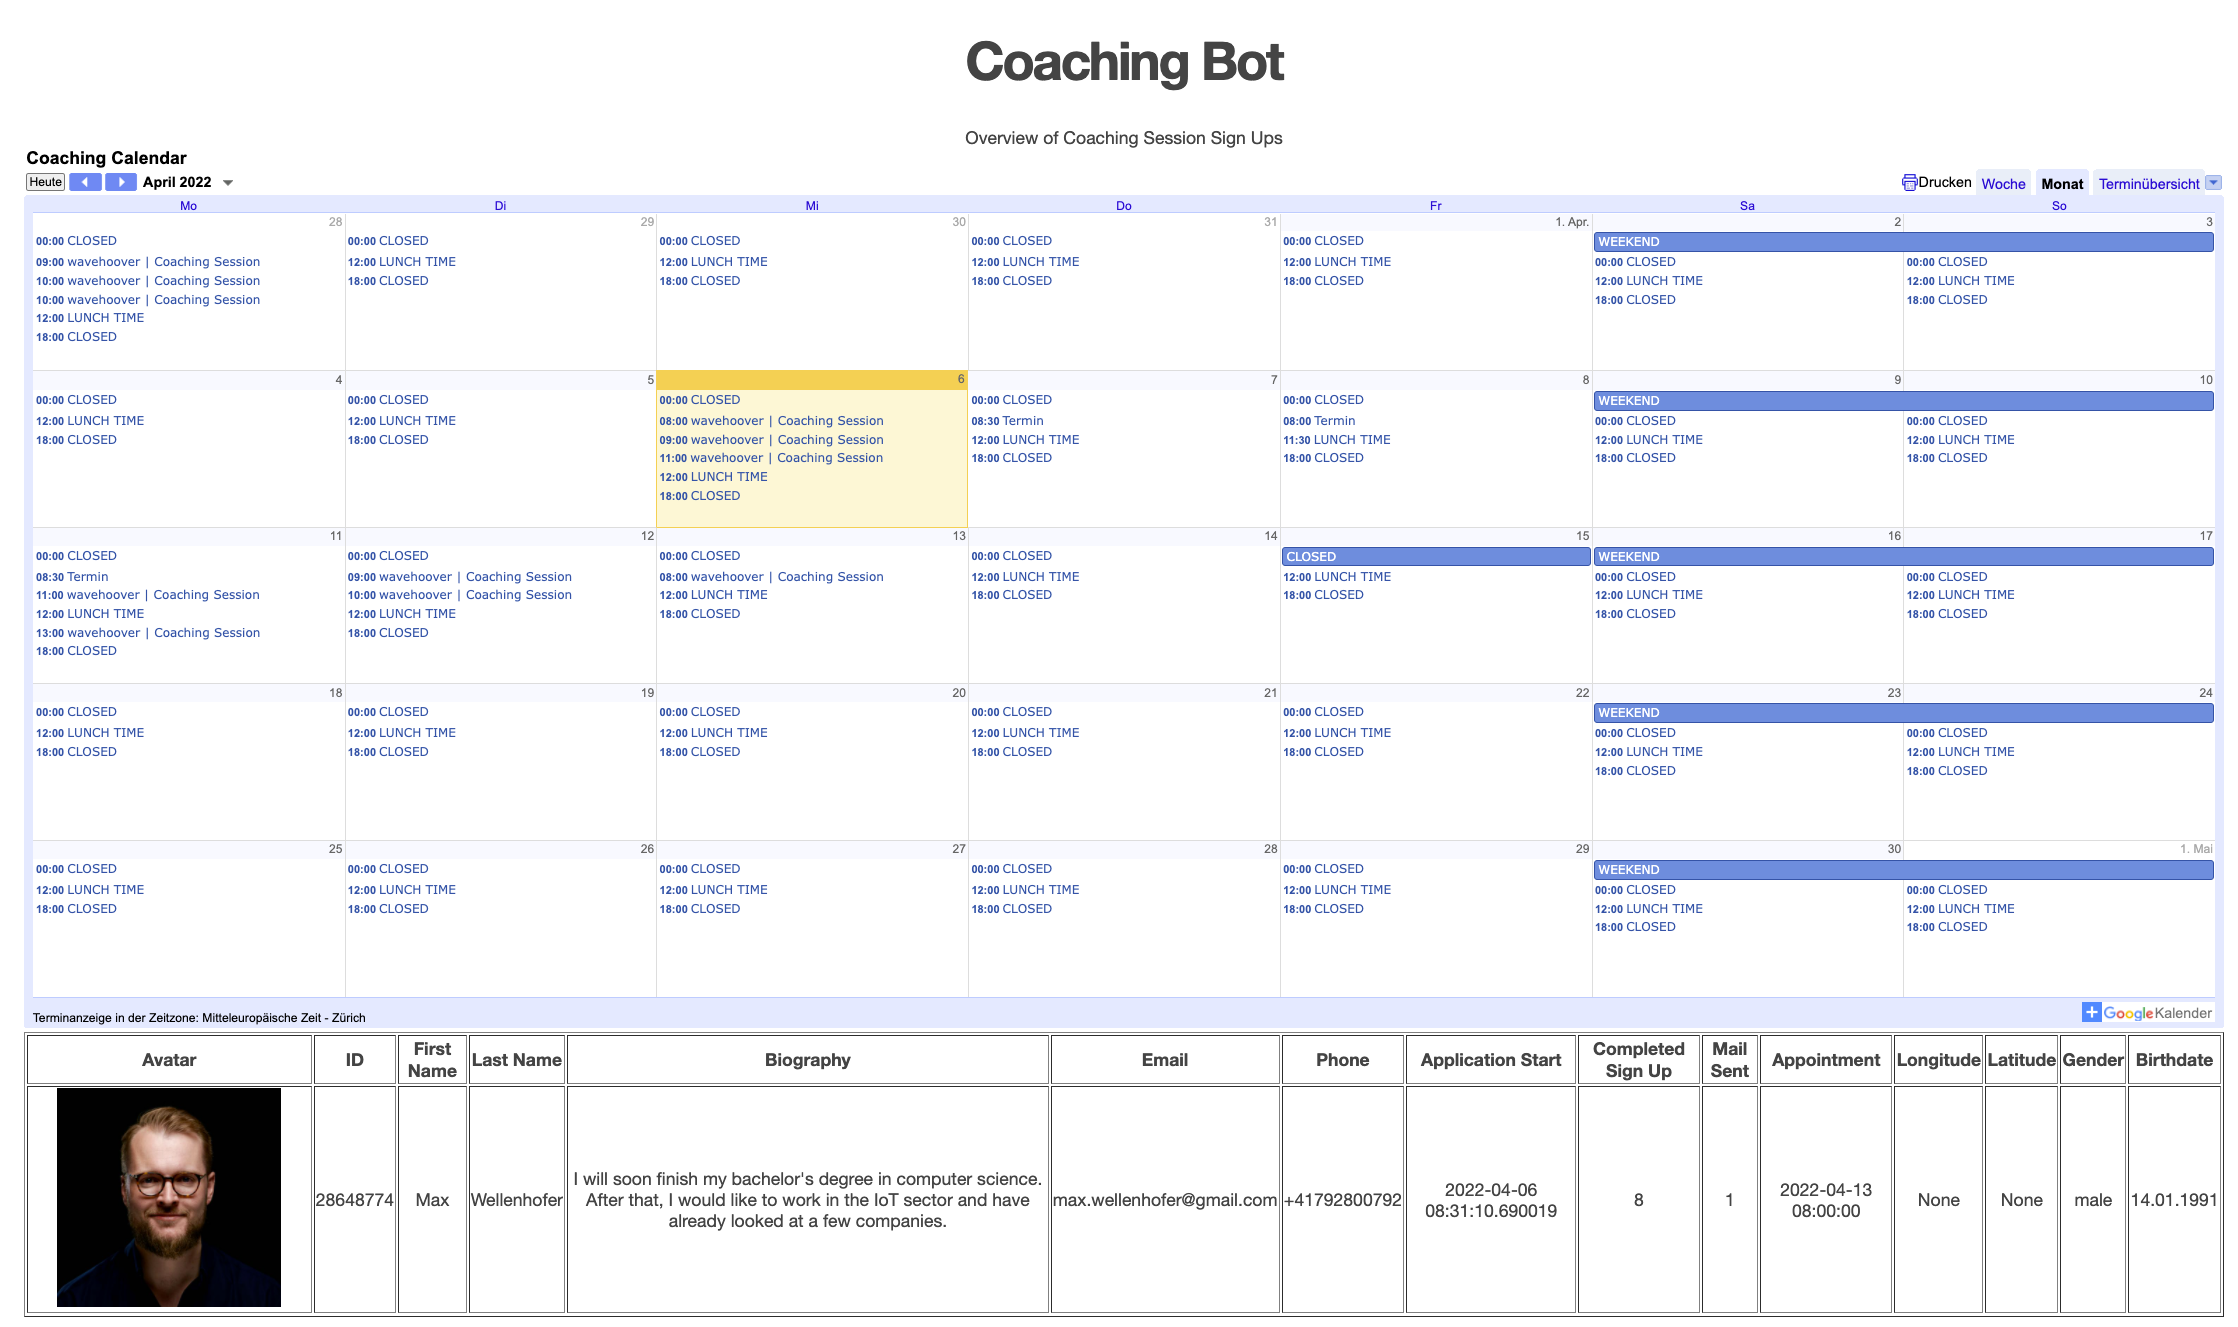
\includegraphics[width=1\textwidth]{images/Screenshots/web-gui.png}
		\caption{Coach-Übersicht mit Kalender und Nutzer-Informationen im Listenformat}
		\label{fig: scs..web-gui}
	\end{figure}

